% !TEX root = main.tex
\documentclass[english,a4paper,12pt,twoside,table]{memoir}
\usepackage{amsmath}
\usepackage{lipsum}
\newtheorem{lemma}{Lemma}
\usepackage[draft,english]{fixme}
\usepackage[export]{adjustbox}
\usepackage{enumitem}
%\usepackage{pgfplots}
\usepackage{nomencl}
\makenomenclature
\newcommand{\nomunit}[1]{%
  \renewcommand{\nomentryend}{\hspace*{\fill}[#1]\nolinebreak\hspace*{2cm}\mbox{}}%
}

\usepackage{babel}
\usepackage{slantsc}
\usepackage{array}
\usepackage{pdfpages}

%\setkomafont{subsection}{\usefont{T1}{fvm}{m}{n}}
%\setkomafont{section}{\usefont{T1}{fvs}{b}{n}\Large}
%\setcounter{secnumdepth}{0}
%\pagestyle{empty}


\usepackage{graphicx}		%Tillader indsættelse af billeder
\usepackage{dcolumn}		%Bruges til at lave matematiske tabelsøjler... se datatabel
\usepackage{mathtools}		%Ekstra matematik... bare lad den være, du får muligvis brug for den.
\usepackage{siunitx}
\sisetup{mode=text,range-phrase = {\text{~to~}}}
\usepackage{microtype}
%\usepackage{amssymb}
\usepackage{rotating}
\usepackage{ar}
\usepackage{tcolorbox}
\usepackage{subcaption}

% ting til memoir
\setlrmarginsandblock{4.2cm}{*}{1}
\setulmarginsandblock{3.5cm}{*}{1}
\setheadfoot{2\onelineskip}{\footskip}
\checkandfixthelayout

% gør at subsections også nummeres
\setsecnumdepth{subsection}

\setcounter{tocdepth}{1}

%%%%%%
% ABSTRACT STYLE
%%%%%%
\makechapterstyle{abstract}{
  \renewcommand*{\printchaptername}{}
%  \renewcommand*{\chapnumfont}{\normalfont\sffamily\huge\bfseries}
  \renewcommand*{\printchapternum}{
    \flushleft
    \begin{tikzpicture}
      \draw[fill,color=black] (0,0) rectangle (2cm,2cm);
      \draw[color=white] (1cm,1cm) node { \chapnumfont\thechapter };
    \end{tikzpicture}
  }
 % \renewcommand*{\chaptitlefont}{\normalfont\sffamily\Huge\bfseries}
  \renewcommand*{\printchaptertitle}[1]{\center\chaptitlefont\Large##1}
}
%%%%%%

%%%%%%
% PAGESTYLE
%%%%%%
\makepagestyle{main}
\makepsmarks{main}{
  \createmark{chapter}      {both}{shownumber}{}{. \ }
  \createmark{section}      {both}{shownumber}{}{. \ }
  %\createmark{subsection}   {both}{shownumber}{}{. \ }
  % \createplainmark{toc}     {both}{\contentsname}
  % \createplainmark{lof}     {both}{\listfigurename}
  % \createplainmark{lot}     {both}{\listtablename}
  % \createplainmark{bib}     {both}{\bibname}
  % \createplainmark{index}   {both}{\indexname}
  % \createplainmark{glossary}{both}{\glossaryname}
}
\makeoddhead{main}{}{}{\rightmark}
\makeevenhead{main}{\leftmark}{}{}
% sidens fod: sidetal
\makeoddfoot{main}{}{}{\thepage}
\makeevenfoot{main}{\thepage}{}{}
% smid en linie under
\makeheadrule{main}{\textwidth}{\normalrulethickness}

% \setsecheadstyle{\large\bfseries\raggedright}
% \setsubsecheadstyle{\normalsize\bfseries\raggedright}

\nouppercaseheads
\pagestyle{main}
%%%%%%

%%%%%%
% CHAPTER PAGE STYLE
%%%%%%
% \makeoddhead{plain}{}{}{}
% \makeevenhead{plain}{}{}{}
% % sidens fod: sidetal
% \makeoddfoot{plain}{}{}{\thepage}
% \makeevenfoot{plain}{\thepage}{}{}
% \aliaspagestyle{chapter}{plain} % make chapter pages same page style as everything else


%%%%%%
% CHAPTER STYLE
%%%%%%
%\usepackage[table]{xcolor}
\usepackage{tikz}

\makechapterstyle{box}{
  \renewcommand*{\printchaptername}{}
%  \renewcommand*{\chapnumfont}{\normalfont\sffamily\huge\bfseries}
  \renewcommand*{\printchapternum}{
    \flushleft
    \begin{tikzpicture}
      \draw[fill,color=black] (0,0) rectangle (2cm,2cm);
      \draw[color=white] (1cm,1cm) node { \chapnumfont\thechapter };
    \end{tikzpicture}
  }
 % \renewcommand*{\chaptitlefont}{\normalfont\sffamily\Huge\bfseries}
  \renewcommand*{\printchaptertitle}[1]{\flushleft\chaptitlefont##1}
}
%%%%%%


% used for flow charts
\usetikzlibrary{shapes,arrows}
% Define block styles
\tikzstyle{decision} = [diamond, draw, fill=blue!10,
    text width=9em, text badly centered, node distance=3cm, inner sep=0pt]
\tikzstyle{block} = [rectangle, draw, fill=blue!10,
    text width=10em, text centered, rounded corners, minimum height=4em]
\tikzstyle{line} = [draw, -latex']

\usepackage{booktabs}
\setlength{\heavyrulewidth}{0.15em}
\setlength{\lightrulewidth}{0.08em}

% Where to look for figures
\graphicspath{ {./figures/} }

\newcommand{\mc}[1]{\multicolumn{1}{c}{#1}}
%\usepackage{threeparttable}
%\usepackage{multirow}

\numberwithin{equation}{chapter}
\numberwithin{table}{chapter}
\numberwithin{figure}{chapter}
\usepackage{varioref}
\usepackage[hidelinks]{hyperref}
\usepackage[draft]{fixme}
\linespread{1.15}
\usepackage[sc]{mathpazo}
\usepackage{wasysym}
\usepackage{cite}
\usepackage{multirow}
\usepackage{capt-of}

\parindent 0pt
\setlength{\parskip}{2mm plus0mm minus0mm}

% Included chapters
\includeonly{
introduction,
vehicleperformance,
airfoils,
conceptdesign,
experiment,
simulation,
construction,
discussion,
conclusion,
perspective,
media,
appendices
}


% Macros
\newcommand{\sref}[1]{Section~\ref{#1}}
\renewcommand{\fref}[1]{Figure~\ref{#1}}
\renewcommand{\tref}[1]{Table~\ref{#1}}
\renewcommand{\eqref}[1]{Equation~(\ref{#1})}
\renewcommand{\vec}[1]{\mathbf{#1}}
\newcommand{\half}[0]{\frac{1}{2}}
\newcommand{\mean}[1]{\ensuremath{\left\langle #1 \right\rangle}}
\newcommand{\pdiff}[2]{\frac{\partial #1}{\partial #2}} % Partial derivative
\newcommand{\ppdiff}[2]{\frac{\partial^2 #1}{\partial #2^2}} % Partial derivative
\newcommand{\mat}[1]{\ensuremath{\boldsymbol{#1}}}
\newcommand{\norm}[1]{|#1|}
\newcommand{\cov}[0]{\text{cov}}
\newcommand*\chem[1]{\ensuremath{\mathrm{#1}}}

\usepackage{listings}
\usepackage{color}
\usepackage{textcomp}
\definecolor{listinggray}{gray}{0.9}
\definecolor{lbcolor}{rgb}{1,1,1}
\lstset{
	backgroundcolor=\color{lbcolor},
	tabsize=2,
	rulecolor=,
	language=matlab,
        basicstyle=\scriptsize,
        upquote=true,
        aboveskip={1.5\baselineskip},
        columns=fixed,
        showstringspaces=false,
        extendedchars=true,
        breaklines=true,
        prebreak = \raisebox{0ex}[0ex][0ex]{\ensuremath{\hookleftarrow}},
        frame=single,
        showtabs=false,
        showspaces=false,
        showstringspaces=false,
        identifierstyle=\ttfamily,
        keywordstyle=\color[rgb]{0,0,1},
        commentstyle=\color[rgb]{0.133,0.545,0.133},
        stringstyle=\color[rgb]{0.627,0.126,0.941},
}
%%%%% BEAUTIFUL TABLES %%%%%
\usepackage{xcolor}
\definecolor{seablue}{HTML}{4C72B0}
\definecolor{seagreen}{HTML}{55A868}
\definecolor{seared}{HTML}{C44E52}
\definecolor{seapurple}{HTML}{8172B2}
\definecolor{seayellow}{HTML}{CCB974}
\definecolor{seacyan}{HTML}{64B5CD}
\usepackage{tabularx}

\renewcommand{\arraystretch}{1.5}
\setlist{nolistsep}

%%% Makes fonts work
\usepackage[cmintegrals,cmbraces]{newtxmath}
\usepackage{ebgaramond}
\usepackage[T1]{fontenc}

%%%%% BEGIN DOCUMENT %%%%%
\begin{document}
\pagenumbering{roman}
\pagestyle{plain}
%% !TEX root = main.tex
%% BOS FORSIDESKABELON
\begin{titlingpage}

\begin{center}

\vspace*{0cm}
\HUGE
\textsc{design of rear wing of an electric race car}\\
\vspace{1.5cm}

%\vspace{3cm}
\makebox[\textwidth][c]{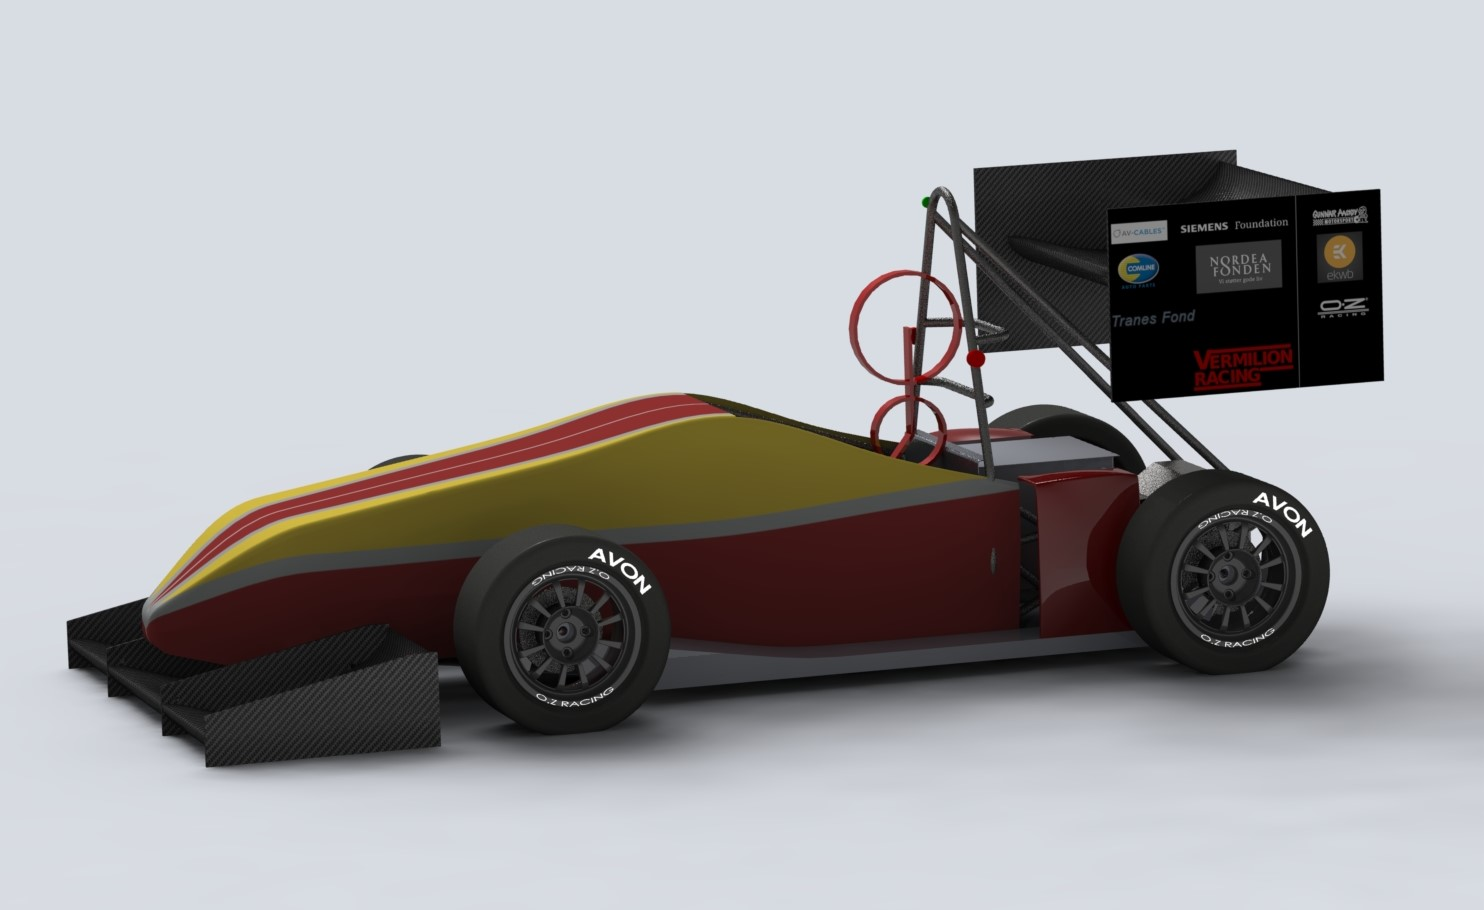
\includegraphics[width=0.7\textwidth]{EveeRender}}%
\vspace{1.2cm}

\large
{
  Steffan Johan Kirk -- S170816\\
    Carl-Emil Grøn Christensen -- S170817\\
    Department of Mechanical Engineering, Technical University of Denmark
}
\vspace{1.5cm}

{
  Supervisor:\\
  Jens Walther\\
  Department of Mechanical Engineering, Technical University of Denmark
}

\vspace{1.5cm}
{August 2018}\\


\end{center}

%\newpage

%%%%%
% The back of the frontpage
%%%%%
%colophon

\end{titlingpage}

\includepdf[pages={1}]{frontpage.pdf}
\setcounter{page}{3}
% !TEX root = main.tex
\chapter*{Acknowledgements}

We would like to thank our supervisors Jens Walther and Robert Mikkelsen, who allowed us to learn intricate details about our own personal project. A special thanks to everyone on the team of Vermilion Racing, who in less than a year managed to take a dream and make it reality. Vermilion Racing is going to compete at the Silverstone race track the 10\textsuperscript{th} of July, where all of our ideas and designs are going to be tested to the limit.

Thanks to Rasmus Himborg from Philips Lighting Denmark, for helping us machine a 1/4 scale wing used in the wind tunnel tests.

Thanks to Bo Tranberg and Jacob Buch for assisting with graphical setup of the report and making sure our figures are beautiful.

Thanks to Nicolai Boertmann and Daniel Rasmussen for the help building the composite wings.

Thanks to DTU Skylab, and especially Martin Meister, Rasmus Bruun, Ralle Malone and Tonja Kramer for always having the time to help us when things looked most dire.

Lastly, a thank to Nenad Mijatovic. Nenad is the overall supervisor for Vermilion Racing and is a significant reason we recently became a DTU Blue Dot project - a highly prestigious title that will ensure that the team will survive for many years to come.

\begin{figure}
  \makebox[\textwidth][c]{
\includegraphics[width=1.5\textwidth]{sponsorstack}}
  \label{fig:sponsorstack}
\end{figure}

% !TEX root = main.tex
\chapter*{Acknowledgements}

We would like to thank our supervisors Jens Honore Walther and Robert Flemming Mikkelsen, for giving us the opportunity to learn intricate details about our own personal project. A special thanks to everyone on the team of Vermilion Racing, who in less than a year managed to make a dream reality. Vermilion Racing is going to compete at the Silverstone race track the 10\textsuperscript{th} of July, where all of our ideas and designs are going to be tested to the limit.

The sponsors who made this project possible are all found on the following page. A big thanks goes out to everyone who supported us and assisted us in creating this project.

Thanks to Rasmus Himborg and Philips Lighting Denmark, for helping us machine a 1/4 scale wing used in the wind tunnel tests.

Thanks to Daniel Rasmussen, Bo Tranberg and Jacob Buch for assisting with graphical layout of the report.

Thanks to Nicolai Boertmann and Daniel Rasmussen for the help building the composite wings.

Thanks to DTU Skylab, and especially Martin Meister, Rasmus Bruun, Ralle Malone and Tonja Kramer for always having the time to help us when things looked most dire.

Lastly, a thank to Nenad Mijatovic. Nenad is the overall supervisor for Vermilion Racing and is a significant reason we recently became a DTU Blue Dot project - a highly prestigious title that will ensure that the team will survive for many years to come.

\begin{figure}
  \makebox[\textwidth][c]{
\includegraphics[width=1.5\textwidth]{sponsorstack}}
  \label{fig:sponsorstack}
\end{figure}

% !TEX root = main.tex
\chapterstyle{abstract}
\vspace{6cm}
\chapter*{Abstract}

The ability to aerodynamically improve grip without adding a weight penalty is key to winning with race cars. High downforce is highly sought after, and the newly started Vermilion Racing Team at DTU is no exception. This work presents the theoretical arguments showing why downforce is important and numerical simulations to optimize the proposed rear wing dimensions. The numerical simulations are held up against a wind tunnel experiment, showing how misalignment of wings can greatly interfere with airflows, confirming the complexity of designing aerodynamical parts. The result is a design specifications of an easily producible rear wing with two elements and large end plates providing an improvement in cornering speeds between $3-35\%$, depending on the turn radius.

\chapterstyle{box}

% !TEX root = main.tex

\nomenclature{$A$}{Frontal area or planform area}%
\nomenclature{$F_x$}{Sum of forces in $x$ direction}
\nomenclature{$m$}{Mass}
\nomenclature{$x$}{$x$-position}
\nomenclature{$\dot{x}$}{Velocity in $x$-direction}
\nomenclature{$\dot{\dot{x}}$}{Acceleration in $x$-direction}
\nomenclature{$C_d$}{Drag coefficient of air resistance}
\nomenclature{$\rho$}{Fluid Density}
\nomenclature{$P$}{Motor effect}
\nomenclature{$F_\text{centripetal}$}{Centripetal force}
\nomenclature{$F_\text{friction}$}{Force due to friction}
\nomenclature{$F_\text{normal}$}{Normal force}
\nomenclature{$\mu$}{Friction coefficient}
\nomenclature{$C_L$}{Lift coefficient}
\nomenclature{$C_l$}{Lift coefficient for 2D airfoils}
\nomenclature{$r$}{Turn radius}
\nomenclature{$g$}{Force due to gravity}
\nomenclature{$u_\infty$}{Velocity of fluid}
\nomenclature{$l$}{Lift force per unit width}
\nomenclature{$L$}{Lift force}%\nomenclature{$L$}{Characteristic length of item (Reynolds number)}
\nomenclature{$\alpha$}{Angle of attack}
\nomenclature{AOA}{Angle of Attack}
\nomenclature{$C_{L_\alpha}$}{DONT KNOW HELP\fxnote{fix this}}
\nomenclature{$\alpha_0$}{Effective angle of attack due to airfoil camber}
\nomenclature{$\AR$}{The effective aspect ratio of the wing}
\nomenclature{$F_d$}{Drag force}
\nomenclature{$C_{d_\text{induced}}$}{Drag coefficient of induced drag}
\nomenclature{$C_D$}{Total drag force}
\nomenclature{$\epsilon$}{Wing tip geometry constant}
\nomenclature{$\AR_\text{actual}$}{The actual aspect ratio of the wing}
\nomenclature{$h$}{Height of end plate}
\nomenclature{$b$}{width of the wing}
\nomenclature{$c$}{Chord length}
\nomenclature{PDS}{Product Design Specification}
\nomenclature{$\text{Re}$}{Reynolds number}
\nomenclature{$\text{Eu}$}{Eulers number}
\nomenclature{$\nu$}{Kinematic viscosity}
\nomenclature{$u_m$}{Fluid velocity of model}
\nomenclature{$L_m$}{Characteristic length of model}
\nomenclature{$E$}{Young's Modulus}
\nomenclature{$I$}{Second moment of inertia}
\printnomenclature


%%%%% Signature page
\newcommand{\namesigdate}[2][5cm]{%
  \begin{tabular}{@{}p{#1}@{}}
    #2 \\[2\normalbaselineskip] \hrule \\[0pt]
    {\small \textit{Signature}} \\[2\normalbaselineskip] \hrule \\[0pt]
    {\small \textit{Date}}
  \end{tabular}
}

\newpage\thispagestyle{empty}\mbox{}\newpage
\tableofcontents*
%\newpage\thispagestyle{empty}\mbox{}\newpage
\newpage
\pagenumbering{arabic}
\setcounter{page}{1}
\pagestyle{main}

%%%%% INCLUDE CONTENT FILES %%%%%

%\include{filename}
% !TEX root = main.tex
\chapter{Introduction}
Drag, lift and side force. Those are the three cornerstones to vehicle aerodynamics, which dictate how a car acts. Inverted wings serves as perfect agents to create negative lift, also known as downforce.

- Initial thought would be to reduce drag in order for the car to move as smoothly as possible. \cite{jkatz}\\
- Downforce increases tires' cornering and acceleration abilities. Higher downforce gives better grip.\\
- Downforce is like having extra weight pressing down on the wheels without the extra weight penalty. The Hannah Montana deal.

% !TEX root = main.tex
\chapter{Aerodynamic Effects on Vehicle Performance}

  The first argument to the importance of aerodynamics is based around two facts: The fact that drag is neglible in regards to the Formula Student vehicle's top speed on straights, and the fact that aerodynamically increasing the vehicle's \emph{effective} mass due to downforce increases tyre grip, which in turn allows for higher cornering velocities.

  The second part of this chapter covers the importance of centering the effective mass increase due to aerodynamic devices close to the center of gravity -- otherwise handling characteristics becomes a function of velocity.

\section{Drag Effects on Straights}
\label{sec:topspeed}

  First, let's explain what makes a car fast, and what parameters we can change to improve the speed of our car.\fxnote{introduce a figure with drag and lift to show what's going on}. The car's acceleration can be described by Newton's second law as:\fxnote{stort D eller lille d i ligningen?}
  \begin{align}
    \sum F_x &= m \ddot{x} = F
    \intertext{Where the sum of forces in the x-direction (the direction of travel) can be expressed as the force already pertained by the vehicle, minus the drag force:}
    F &- C_D \left(\frac{1}{2}  \rho \dot{x}^2 A \right) = m \ddot{x}
    \intertext{Where $C_D$ is the drag coefficient of the vehicle, $\rho$ is the density of the fluid it moves in and $A$ is frontal area of the vehicle. Assuming we're moving at a steady speed, the acceleration is 0, hence}
    F &= C_D \left(\frac{1}{2}  \rho \dot{x}^2 A \right)
    \intertext{As we were interested in the speed of the car, let's solve for the velocity. The force is given by $F = \frac{P}{\dot{x}}$, where $P$ is the power of the car, which gives:}
    \dot{x} &= \left( \frac{2 P}{C_D \left(\rho A \right)}\right)^{\frac{1}{3}}
  \end{align}
  This is assuming we're traveling at terminal velocity -- that is, the point where the $\text{Driving Force} = \text{Friction Force}$. The terminal velocity of the racer is then easily calculated, as the competition restricts the maximum amount of power to $\SI{80}{\kilo\watt}$, and the frontal area of the car is approximated from the CAD drawing seen in figure \ref{fig:frontarea}\fxnote{fix calculation to use 0.99 instead of 1.2}.

  \begin{figure}
    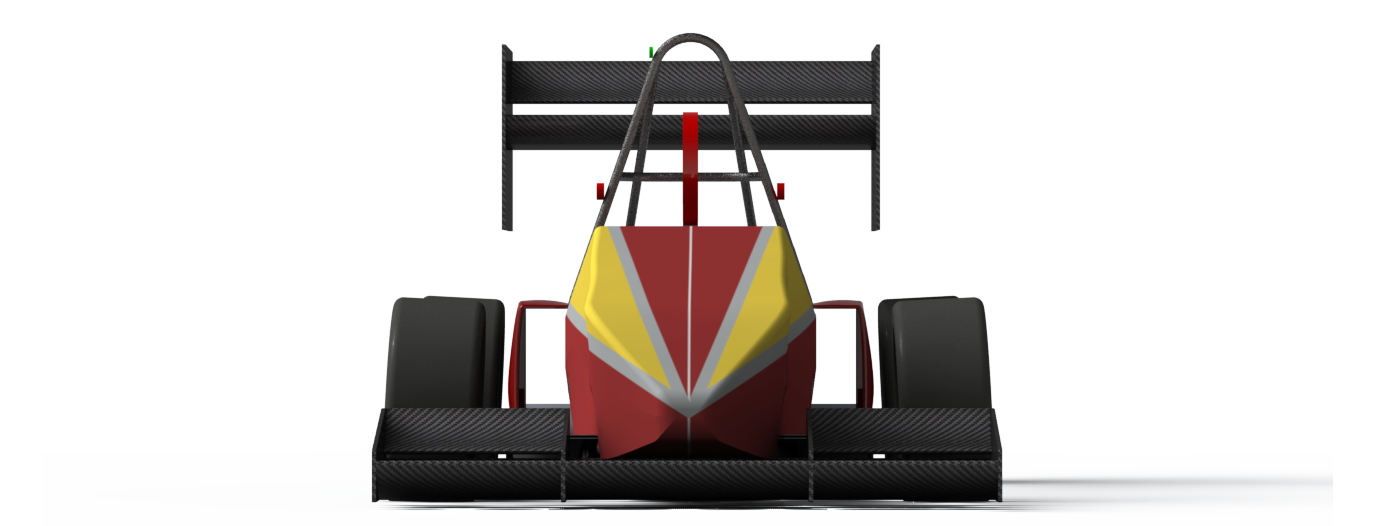
\includegraphics[width=\textwidth]{frontalarea.png}
    \caption{Frontal area of the car with a dummy wing inserted into the CAD model, in order to get an estimate of the drag coefficient $C_D$.}
    \label{fig:frontarea}
  \end{figure}\fxnote{missing radiators}

  \begin{align}
    \dot{x}_\text{max} &= \left(\frac{2\cdot \SI{80}{\kilo\watt}}{0.85\left(\SI{1.225}{\kilogram\per\cubic\metre}~ \SI{1.2}{\square\metre}\right)}\right)^{\frac{1}{3}} = \SI{50}{\metre\per\second} = \SI{181.4}{\kilo\metre\per\hour}
    \intertext{however, given the ruleset a forecasted maximum of $\SI{110}{\kilo\metre\per\hour}$ allows a much larger drag coefficient $C_D$:}
    C_D &= \frac{2 P}{\dot{x}^3 \left(\rho A \right)}
    = \frac{2 \cdot \SI{80}{\kilo\watt}}{(\SI{120}{\kilo\metre\per\hour})^3 \left(\SI{1.225}{\kilogram\per\cubic\metre}~ \SI{1.2}{\square\metre} \right)} = 2.82
  \end{align}\fxnote{insert source}
  Thus, the car's top speed will only be limited by a drag factor $>2.82$, which is far above the drag introduced by the aerodynamic devices.

  From this derivation, it is clear that the car's abilities at maximum speeds far exceed the requirement of the track. Therefore, the next step is to improve cornering speeds which depend strongly on the tyre's grip on the surface of the road \cite{jkatz}.

  \subsection{Downforce Effects on Cornering}

    Shown before, drag does not limit the car's performance on straights. During cornering, drag is not an issue either, but the grip of the tyres limits the maximum velocity before the vehicle loses traction due to the centripetal force which is given by:\cite{taylor2005classical}
    \begin{align}
      F_\text{centripetal} &= \frac{m\dot{x}^2}{r}
      \intertext{where $r$ is the distance to the center of the cornering circle. The frictional force the car exerts due to downforce and tyre grip is given by:}
      F_\text{friction} &= \mu F_\text{normal} \label{eq:downforcetocorneringspeed}
      \intertext{where the normal force is given by both the weight and (negative) lift of the car, which serves as an effective mass increase:}
      F_\text{friction} &= \mu \left(mg + \frac{1}{2}\rho C_L A \dot{x}^2 \right)
      \intertext{The vehicle will lose traction when the frictional force is less than the centripetal force.}
      \frac{m\dot{x}^2}{r} &> \mu \left(mg + \frac{1}{2}\rho C_L A \dot{x}^2 \right)
      \intertext{Giving the maximum velocity for a given corner radius before the car skids out:}
      \Rightarrow \dot{x} &< \left(\frac{2\mu mg r}{m - \mu C_L \rho r  A}\right)^{\frac{1}{2}}
    \end{align}
    Again, the forecasted variation in radii of corners is prescribed by the rules to be between \SIrange{3}{50}{\metre}\cite{FSrules18}. Plotting this for various $C_L$ values between $1.5$ to $2.6$ \cite{CLvalues}, assuming $m=\SI{300}{\kilogram}$, $\mu = 1.5$ \cite{tyrefriction} and $A = \SI{0.99}{\square\metre}$ as previously used. The result can be seen in figure \ref{fig:cornerspeedvslift}.
    \begin{figure}
      \makebox[\textwidth][c]{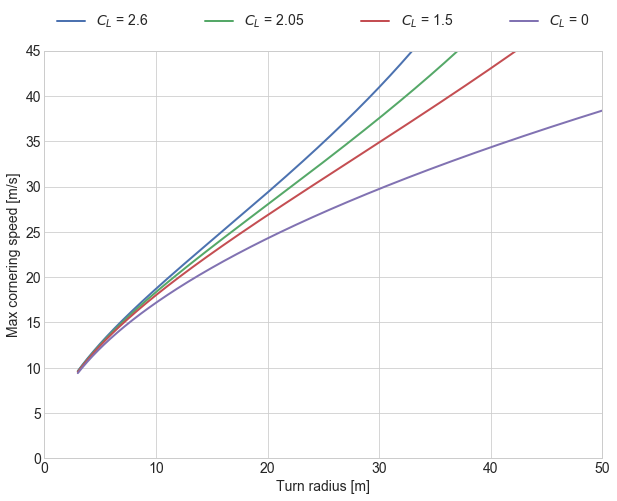
\includegraphics[width=1.2\textwidth]{turnspeedperCL2}}%
      \caption{Cornering speed as a function of turn radius for various lift coefficients.}
      \label{fig:cornerspeedvslift}
    \end{figure}

\subsection{Load Distribution}

  The scope of this thesis is not to incorperate a full aerodynamic package, but a quick overview of load distribution is essential to understanding the behaviour of the car.

  The effective mass added from negative lift depends on the lift coefficient. It is evident that different items on the car carry different lift coefficients, thus making the lifting forces over the cars length a function of relative speed. For the unexperienced driver, this is not easily managed as handling characteristics change with velocity. Therefore, it is desirable to have the aerodynamic center of pressure close to the car's center of gravity, in order to have similar handling at all velocities. While this is not handled in this thesis, it is ideal for future iterations and essential for a full aerodynamical package.

%Check https://uta-ir.tdl.org/uta-ir/bitstream/handle/10106/24176/Merkel_uta_2502M_%2012503.pdf?sequence=1

% !TEX root = main.tex
\chapter{Airfoils and Inverted Wings}

Achieving a large negative lift coefficient $C_L$ can be done in many ways. Inspecting race cars throughout the years show that airfoils have been used as early as 1966 when Jim Hall attached a rear wing to his Chaparral 2E \cite{hucho}. Since then, the inverted wings have been a staple in the racing industry with various three dimensional geometries affecting the overall performance even further.

This chapter covers the pressure distribution of various airfoils, the selection criterions of the competition, three dimensional geometrical effects and the tools of the optimization trade.

\section{Airfoil theory}

  An airfoils is the 2-dimensional cross section of a wing, that's characteristic of the wing's lifting characteristics. It is important to know the nomenclature: The leading edge is  the most forward point of the wing, the trailing edge is the most rearward point of the wing. Camber is how much the wing ''flexes''.




  \fxnote{Mostly laminar flow, boundary layer mustn't trip or create bubbles,}
Theory of airfoils from katz book, to be written tuesday 19.



  \subsection{Pressure distribution}


  \fxnote{Where does downforce come from? Where does drag come from?}

  \subsection{Lift and Drag Coefficient}

  \subsection{Which parameters does an airfoil have? What can we change}

  \subsection{Angle of Attack}

  \subsection{Ground Effects}\fxnote{unsure}

  \subsection{Aspect Ratio and End Plates}

    An important identifyer when describing the entire wing is, apart from chord length and airfoil design, the width. The definition used for describing the physical span is called Aspect Ratio, and for a rectangular wing is:
    \begin{align}
        \AR_\text{actual} &= \frac{b}{c}
        \label{eq:ARactual}
    \end{align}
    The end plates adds a virtual additional length, by reducing the vortices that usually go around the wing and reduce lift. A corrected aspect ratio can be found for wings with side plates as:
    \begin{align}
      \AR &= \AR_\text{actual}\left(1+1.9\frac{h}{b}\right)
    \end{align}
    where $h$ is the height of the end plate, and $b$ is the width of the wing as in equation \ref{eq:ARactual} \cite{jkatz}.

  \fxnote{something about Navier Stokes equations.}

\section{Comparison of Airfoils}
Choosing the MSHD wing.
To be written from MSHD article on tuesday 19.

\section{Multi elements? How many is enough}
From katz book, written tuesday 19.

\section{Optimization Tools}

Also from katz book to be written tuesday 19.

Building physical models is cool, wind tunnel time is expensive though

Let's use CFD!

To make sure CFD works, we need to perform experiments to verify simulations work.

Let's make a small scale wind tunnel test and simulate the rest!

% !TEX root = main.tex
\chapter{Concept Design}

  The following contains the conceptual design of a rear wing based on the previous chapters. First, a walkthrough of different airfoil profiles and their benefits is followed by selection of one particular. Second, analyzing the amount of elements the wing should consists of with regards to production time and ease of construction. Third, the dimensional requirements outlined by the competition rules are given, and finally, a Product Design Specifiation (PDS) is set up to make sure that the design solution addresses all the problems it attempts to solve. Based on the PDS, an initial design is proposed, followed by a section describing the various possible methods of optimization.

  \section{Comparison of Airfoils}

    Finding a fitting airfoil requires deep investigation of airfoil databases and articles. The requirements for this airfoil according to the PDS is a really high lift wing, operating at large ranges of Reynolds numbers, where the highest (according to track regulations) is around:
    \begin{align}
      \text{Re} &= \frac{uL}{\nu} = \frac{\SI{30.56}{\metre\per\second}\SI{0.6}{\metre}}{\SI{1.491E-5}{\metre\squared\per\second}} \approx \SI{1.2E6}{}
      \intertext{to around:}
      \text{Re} &\approx \SI{3E5}{} ~\text{at}~ \SI{15}{\metre\per\second}
    \end{align}
    which is the speed estimated for the tightest corners in the competition \cite{FSrules18}. Thereto, the wanted airfoil should have soft stall characteristics, and be very resilient to laminar separation bubbles (LSB for short. The interested reader is refered to reference \cite{jkatz}). This is done by having a large leading edge radius.

    \begin{figure}
      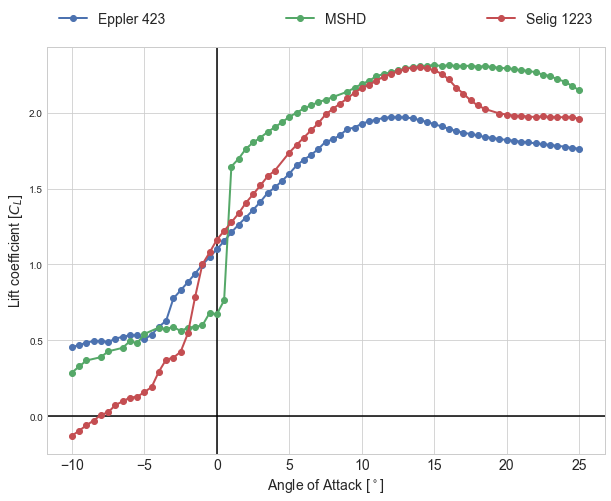
\includegraphics[width=\textwidth]{clperAOAtheory}
      \caption{A comparison of the three airfoils as a function of angle of attack. The MSHD profile shows high lifting characteristics over a wide range of angles of attack. Comparisons are from XFOIL at $\text{Re} = \SI{3E5}{}$.}
      \label{fig:AOAofairfoils}
    \end{figure}

    After a thorough research comparing high lift-low Reynolds number airfoils functioning over a wide variety of angles of attack, three airfoil are selected for further examination. The Eppler E423, the Motor Sport High Downforce (MSHD) and finally the Selig S1223. The lift coefficient can be seen as a function of angle of attack in figure \ref{fig:AOAofairfoils}.

    The MSHD performs incredibly well over a wide range of AOAs, with very low variation in lift coefficients. The MSHD airfoil is designed specifically for the Formula Student competition, which does make the choice rather obvious. The MSHD is selected for further investigation, and will be the airfoil of choice.

    Lastly, finding the right amount of elements depends on the airfoil, and based on the MSHD profile and previous studies, two elements were chosen: A main element and a scaled down flap with $35\%$ of the length of the main element \cite{winginitialangle}. The two elements will have an identical airfoil, as this is a classical way of generating successful multi element wings \cite{sameairfoilgoodidea}. This makes production time shorter, monetary cost lower and (hopefully) provides ample lift for the first generation race car.

  \section{Dimensional Requirements}

    The formula student competition has a clear ruleset dictating the dimensional requirements of aerodynamic devices. The most crucial elements are outlined below:

    \begin{tcolorbox}[colframe=seapurple,colback=seapurple!1]
      Height Restrictions:
      \begin{itemize}
        \item[T7.3.1] All aerodynamic devices rearward of a vertical plane through the rearmost portion of the front face of the driver head restraint support, excluding any padding, set to its most rearward position must be lower than $\SI{1.2}{\metre}$ from the ground.
      \end{itemize}

      Width Restrictions:
      \begin{itemize}
       \item [T7.3.2] All aerodynamic devices higher than 500 mm from the ground, must not extend outboard of the most inboard point of the rear wheel/tire.
      \end{itemize}

      Length Restrictions:
      \begin{itemize}
        \item [T7.3.3] All aerodynamic devices must not extend further rearward than 250 mm from the rearmost part of the rear tires
      \end{itemize}

      Minimum Edge Radii of Aerodynamic Devices:
      \begin{itemize}
        \item[T7.4\hphantom{.0}] All forward facing edges of aerodynamic devices that could contact a pedestrian must have a
      minimum radius of $\SI{5}{\milli\metre}$for all horizontal edges and 3 mm for vertical edges.
      \end{itemize}
      \vspace{5pt}
      \hspace*{\fill}\tiny{Rules from Formula Student UK 2018 ruleset \cite{FSrules18}.}
    \end{tcolorbox}

    The dimensional requirements from the rules was sketched on the front plane of the car's CAD drawing. This allows positioning the wing in the square seen in figure \ref{fig:cadplacement}.

    \begin{figure}
      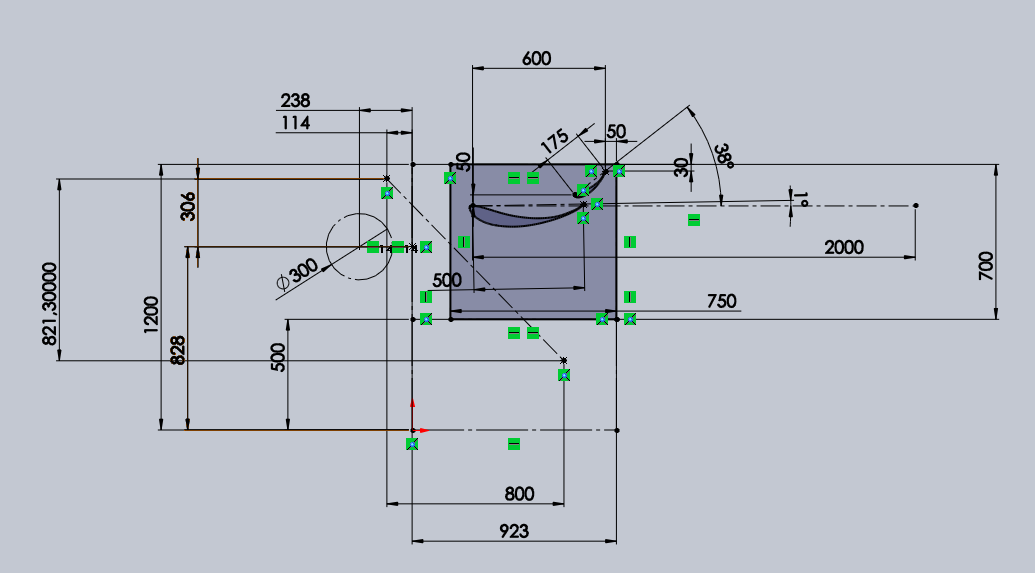
\includegraphics[width=\textwidth]{cadplacement}
      \caption{The ruleset above drawn against the design of the car. The marked square is the area where the wing can be freely placed.}
      \label{fig:cadplacement}
    \end{figure}

  \section{Product Design Specification (PDS)}
  \label{sec:PDS}

    The PDS is a design tool created to ensure that the project solves the problems it set out to. The specifications uncovered in the previous sections are boiled down to their bare essentials, and in order to cover as large a solution space as possible, the PDS contains as few \emph{requirements} as possible. However, fulfilling the requirements is essential for a proper solution. While the criteria are not crucial, the criteria are the difference between an acceptable solution and a good one. The PDS will be revised at the discussion section, in order to verify the design solution fulfills all requirements.
    \begin{table}
      \begin{tabularx}{\textwidth}[t]{>{\columncolor{seapurple!40}}l XX}
      \arrayrulecolor{seapurple}\hline
      \rowcolor{white}
      \textbf{\textcolor{seapurple}{Issue}} & \textbf{\textcolor{seapurple}{Requirement}} & \textbf{\textcolor{seapurple}{Criteria}}\\
      \hline
      Weight & Must not move CM above halfway point & As low as possible \\
      Safety & Must be in compliance with FSAE rules & Should not make handling difficult for driver\\
      Durability & Must have no fatigue limit. Must to be waterproof & \\
      Performance & High downforce \& soft stall characteristic at all speeds & Should retain perfomance despite tripping. Should have end plates.\\
      Dimensioning & Must be within area defined by FSAE rules & Should allow space for motor removal. \\
      Production & Low time- and monetary cost & \\
      \end{tabularx}
      \caption{The PDS table shows how the final design lives up to the proposed specifications.}
    \end{table}
  \section{Initial Design}

    \begin{figure}
      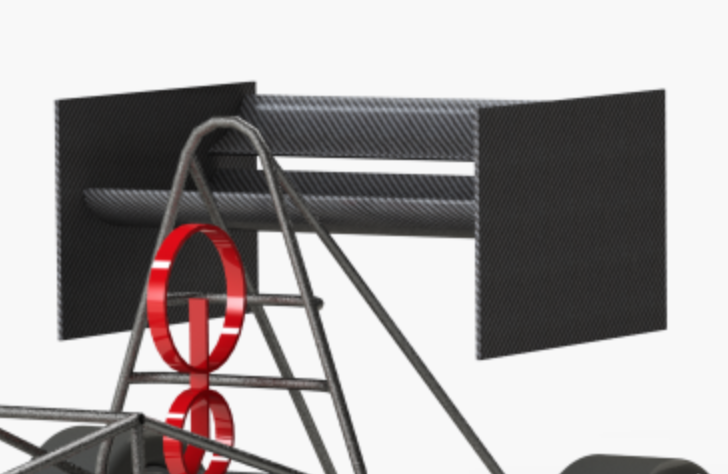
\includegraphics[width=\textwidth]{firstdraftwing1}
      \caption{Initial design of the rear wing based on the PDS and initial research. Optimization of the wing is the next step.}
      \label{fig:firstdraftwing}
    \end{figure}

    An initial design can be made based on the PDS and the design ideas above. The MSHD airfoil has a lot of the wanted characteristics: High downforce, both leading- and trailing edge stalls are soft, and the usable AOA-ranges are high. Furthermore, based on equation \ref{eq:endplates}, we want as large end plates as possible, which will therefore fill the entirety of the allowed area. The dimensional restrictions from the competition are shown in figure \ref{fig:cadplacement}. Finally, two elements are chosen as that gives a large amount of lift over even higher angles of attack, while being cheap timewise to construct.

    A first draft of the design can be seen in \ref{fig:firstdraftwing}. As the wing is intended to be optimized, a few initial assumptions were made. The first element's tail is angled $1^\circ$ below horizontal, and the angle between the two wing elements is $36^\circ$ based on a previous study \cite{winginitialangle}. The same article provides a first guess of the relative size of the two elements, which should be a good start for the optimization process.

  \section{Optimization Tools}

    In order to optimize a design, there is three ways usually employed in aerodynamics.

    Road testing might seem the easiest method of testing, but constructing full-scale rear wing and iterating is very time consuming. Furthermore, in order to measure downforce correctly, suspension vibration, varying weather and such have to be taken into account, and as is the first car that's being produced, there is no car to test on. Lastly, the driver performance is rarely repeatable, thus making actual road testing a time consuming and inaccurate method of testing the wings.

    Wind tunnels is another option. This allows for construction of down-scaled models, as long as Reynolds numbers are scaled accordingly. However, models can also be difficult to produce, and might not reproduce full scale results correctly. Full scale testing is expensive and wind tunnels of that size are rare.

    Lastly, computational fluid dynamics offer a method of testing a wing without actually producing anything physically. Albeit the seemingly great possibilities, computer time is also expensive, and high resolution solutions require very powerful computers \cite{jkatz}. Luckily for us, we have access to the Niflheim Linux supercomputer cluster located at the Department of Physics at the Technical University of Denmark. The supercomputer has a total of 11368 CPU cores, with 235 Teraflops of processing power.

    In order to verify the numerical models applied to the problem, a wind tunnel test will be performed on a 1/4 scale model and be compared to simulations. Post verification, numerical optimization of the wing will follow in Star-CCM+.

% !TEX root = main.tex
\chapter{Wind Tunnel Experiment}

  Verifying the simulated aerodynamic effects is crucial to ensuring the correctness of the numerical analysis. In order to assess the reliability of the previouisly conducted simulations, a physical measurement of the pressure along the down-scaled wing will provide results for comparison. \fxnote{sounds awful. fix}

  Measurements and tests have been carried out at the DTU Wind laboratory's Red wind tunnel with the help of our supervisor Robert Flemming Mikkelsen the 19\textsuperscript{th} to the 20\textsuperscript{th} of June.

\section{Aerodynamical Theory}

  The theories explaining how fluid effects scale between varying wing sizes is explained, in order to justify using a down-scaled model as evaluation to a real size wing.

  \subsection{Similarity of Flows}
  \label{sec:similarflows}

    In order to perform tests on the rear wing, it has to be scaled down to fit inside the wind tunnel. This reduces the physical size of the wing, which under equal circumstances changes the flow around it. In order to correctly emulate the simulated flow inside a wind tunnel, the Reynolds number and Euler number have to be the same, assuming incompressible flows:
    \begin{align}
      \text{Re}_\text{m} &= \text{Re}\\
      \text{Eu}_\text{m} &= \text{Eu}
      \intertext{Mathematically, the Reynolds- and Euler number are defined as:}
      \text{Eu} &= \frac{p_u - p_d}{pv^2}
      \intertext{where $v$ is the characteristic velocity of the flow, $p_u$ denotes upstream pressure, and $p_d$ denotes downstream pressure, and:}
      \text{Re} &= \frac{u L}{\nu}
    \end{align}
    where $u$ is the velocity relative to the object, $L$ is the characteristic length and $\nu$ is the kinematic viscosity of the fluid.

    For a down-scaled model, matching Reynolds- and Euler number requires an increase in velocity, inversely proportional to the increase in length \fxnote{skriv det her ud plx.}

    \begin{align}
      \frac{u_\text{m} L_\text{m}}{\nu} &= \frac{u L}{\nu} \nonumber \\
      \Rightarrow u_\text{m} &= \frac{L}{L_\text{m}} u \label{eq:windtunnelspeed}
    \end{align}

    Given the nature of the competition, the average cornering speeds are around $\SI{55}{\kilo \meter \per \hour} = \SI{15.28}{\metre\per\second}$, which is where downforce is of most importance. As shown in section \ref{sec:similarflows}, the desired velocity in the wind tunnel for the scale model can be found from equation \ref{eq:windtunnelspeed}

    \begin{align*}
      u_\text{m} &= \frac{\SI{0.6}{\metre}}{\SI{0.15}{\metre}} \SI{15.28}{\metre\per\second} = \SI{61.12}{\metre\per\second}
    \end{align*}

    Which in accordance to the range of The Red wind tunnel.

\section{Equipment}

  The equipment required for performing a wind tunnel test can be seen below:
  \begin{itemize}
    \item The Red wind tunnel ($\SIrange{60}{65}{\metre\per\second}$)
    \item 1/4 scale wing
    \item Syringe inserts
    \item Rubber tubing
    \item Pressure transducer
  \end{itemize}

  The instrumentation and the Red wind tunnel is described below, along with a thorough description of the scale wing designed and produced for the experiment.

  \subsection{Instrumentation}

    Instrumentation to perform the experiments were graciously provided to us by DTU Wind Energy. The following contains a description of the wind tunnel, datalogging devices and software used to perform the measurements.

    \subsubsection{The Red Wind Tunnel}

      The red wind tunnel is an open loop wind tunnel located at DTU Lyngby. A picture of the wind tunnel with our supervisor Robert Mikkelsen can be seen in figure \ref{fig:theredwindtunnel}. It measures $\SI{0.5}{\metre} \times \SI{0.5}{\metre} \times \SI{1.3}{\metre}$ in the test section, with a maximum wind speed of \SI{65}{\metre\per\second}. The wind tunnel functions in low Reynolds number, which fits with the chosen MSHD aerofoil.

      \begin{figure}
        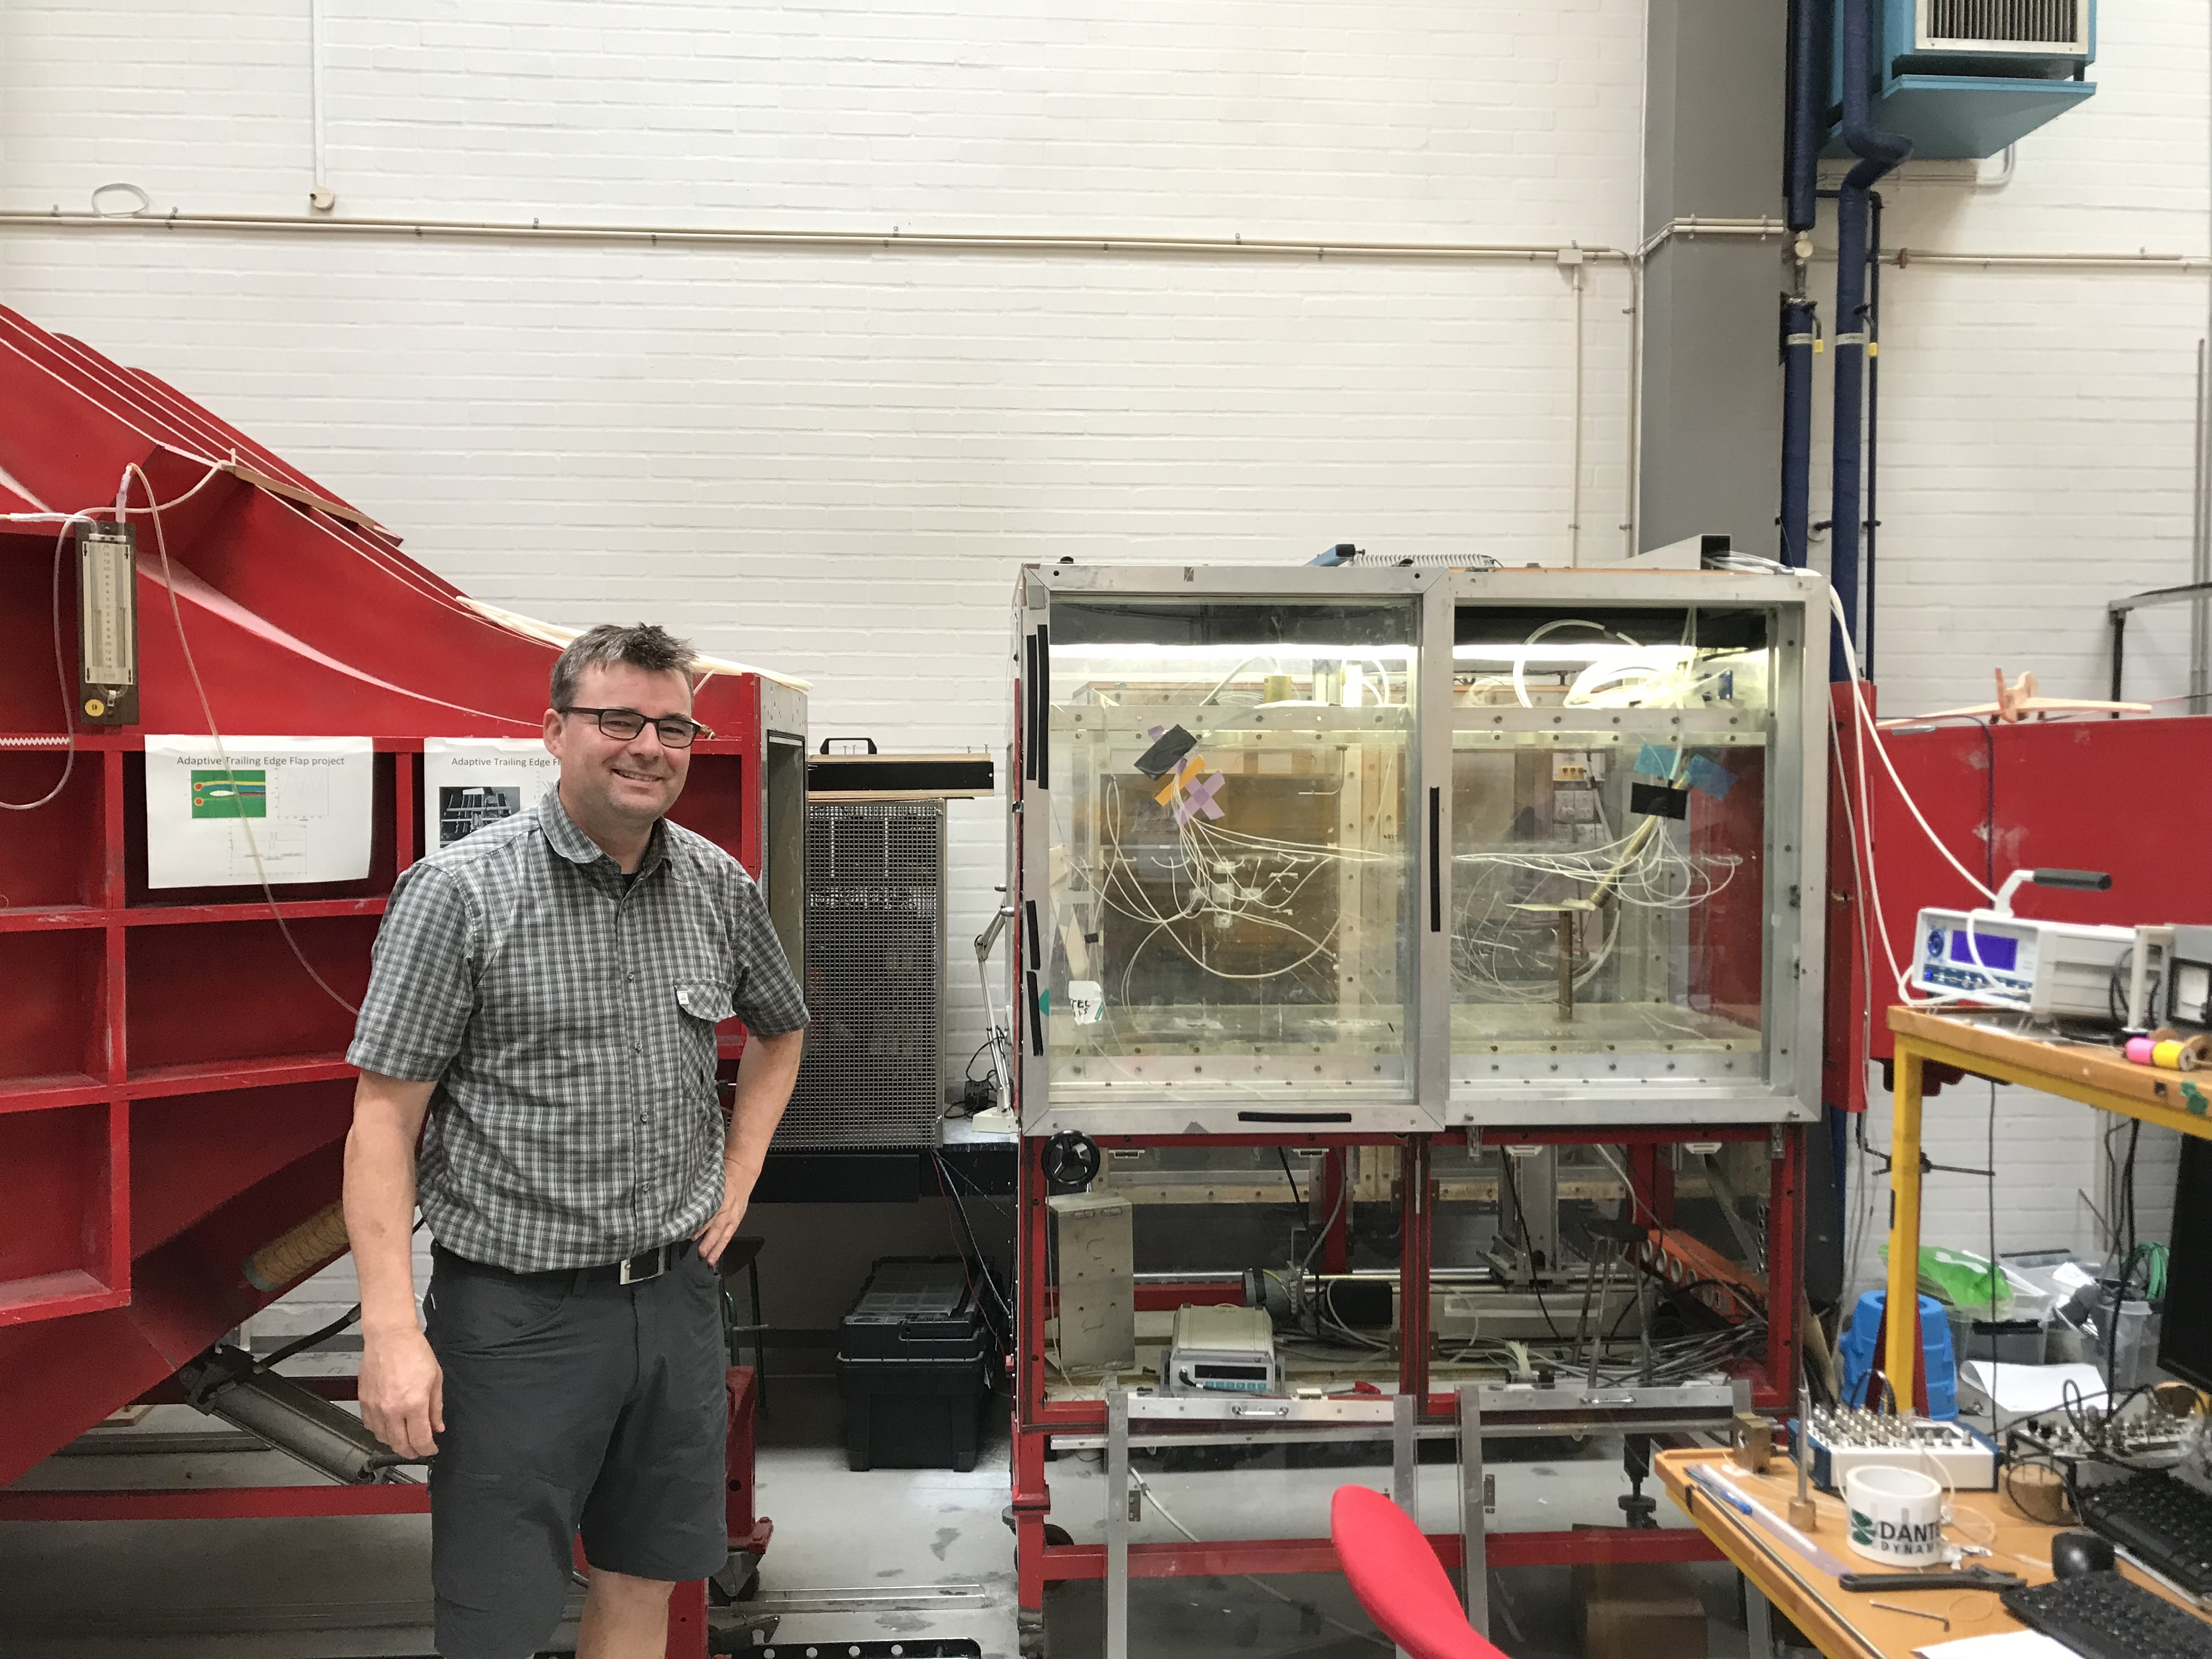
\includegraphics[width=\textwidth]{theredwindtunnel}
        \caption{Robert Mikkelsen posing in front of the Red wind tunnel. To the left is the air inlet, followed by the test section.}
        \label{fig:theredwindtunnel}
      \end{figure}

    \subsubsection{Pressure Measurements}

      The Red wind tunnel is equipped with data logging equipment measuring up to 64 pressure probes on a wing profile, the Angle of Attack (AOA), a force gauge measuring the lift forces, a pitot rake measuring the pressure in the wing's wake, the dynamic pressure in the wind tunnel, the operational speed of the wind tunnel, the air density and the time of measurement. The measurement equipment was connected to a \fxnote{unsure here. Check document} connected to the data-logging software LabVIEW on a nearby computer.

  \subsection{Manufacturing the 1/4 Scale Rear Wing}

    \begin{figure}
      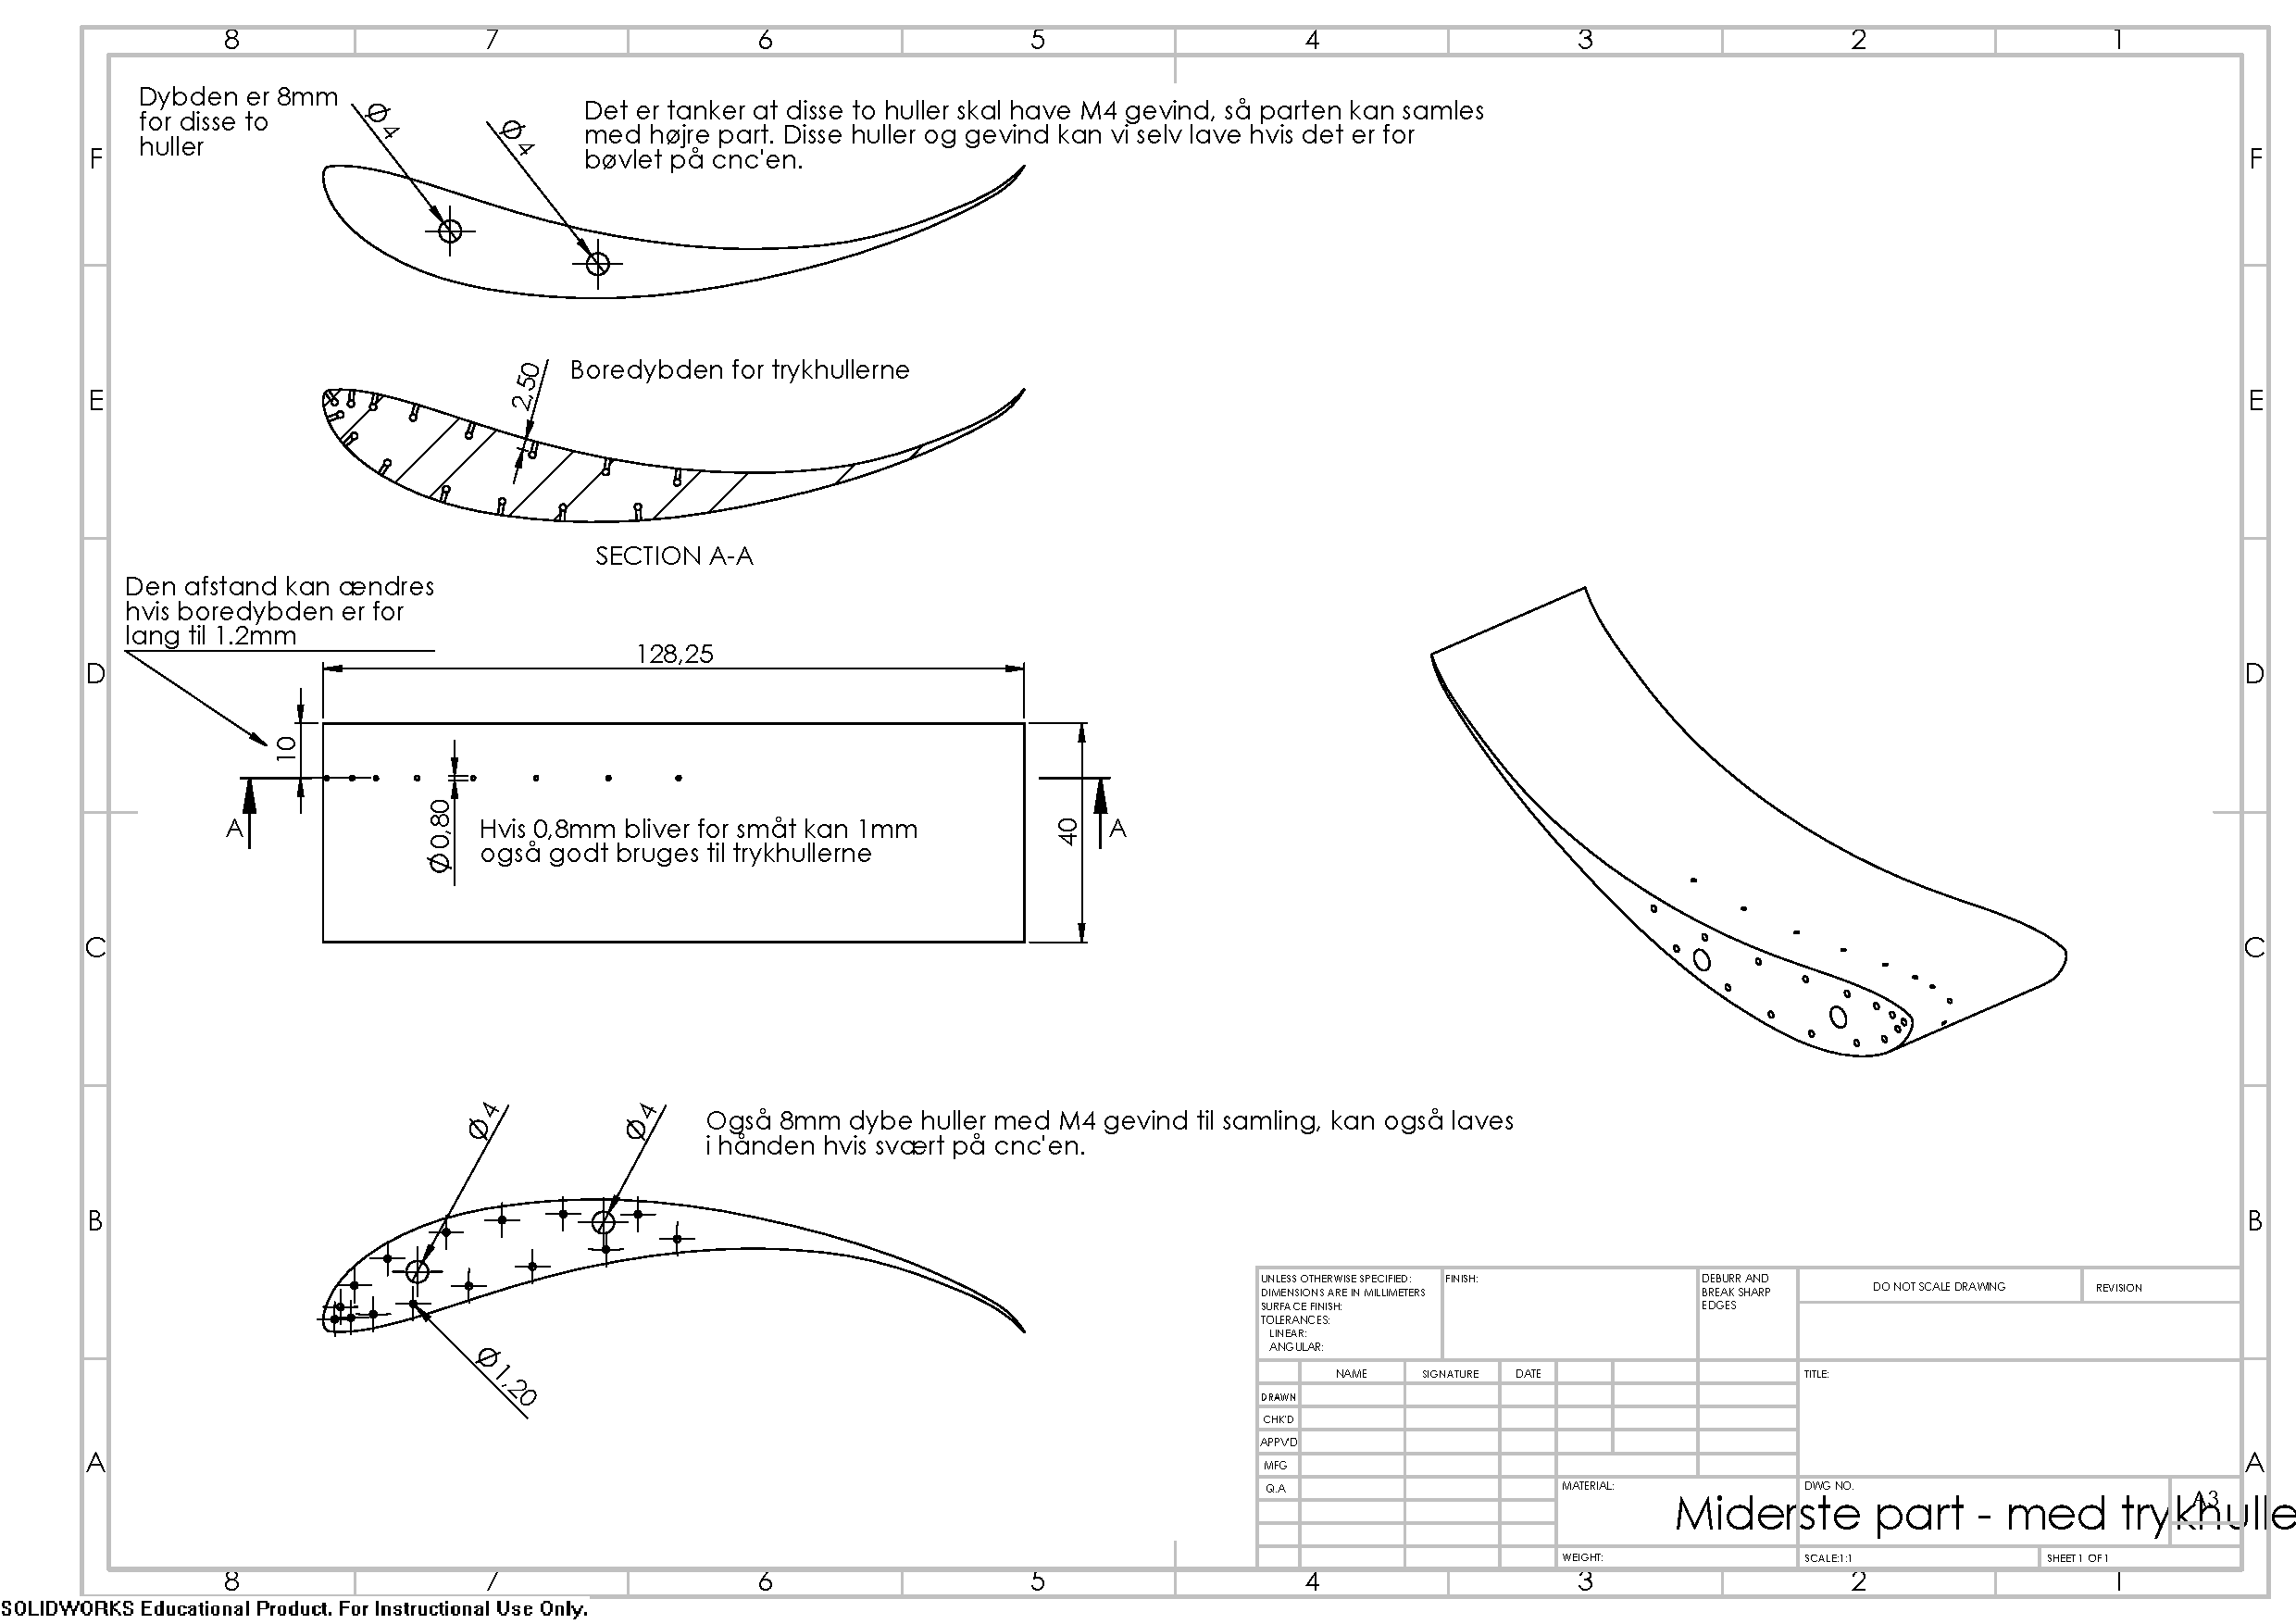
\includegraphics[width=\textwidth,rotate=0]{arbejdstegningvindtunnel}
      \caption{Blueprints of the centerpiece of the wing containing the pressure taps for generating a pressure distribution profile.}
      \label{fig:scalewingblueprint}
    \end{figure}\fxnote{maybe fix blueprint to be more sexy/english}

    \begin{figure}
      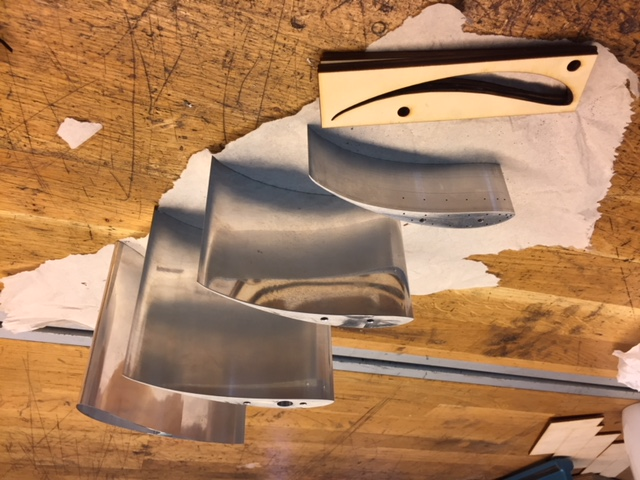
\includegraphics[width=\textwidth, rotate=180]{scalewing}
      \caption{Pieces of the downscaled wing before assembly. Additional H7 holes had to be drilled in order to mount the wing to the force gauge securely.}
      \label{fig:scalewingparts}
    \end{figure}

    After the initial analysis of airfoils, this design was chosen based on preliminary research. From CITE SOMETHING HERE  \fxnote{Insert source}, a rule of thumb for multi element design is that the first element should be around $70\%$ of the total chord length, and the second element around $30\%$. From \cite{jkatz}, the initial position of the elements was chosen. Having the perfect position is not essential, as the experiment is a simply a verification method of the computational method, which will be used to optimize the final deisng.

    The 1/4 scale rear wing was machined at Philips Lighting by Rasmus Himborg based on the technical drawings presented below.

    \subsubsection{Blueprints}

      The wing requires a series of special holes for the measurements needed. 15 holes have to be made along the very narrow wing profile, in order to measure the pressure on the wing's surface. The pressure taps have to be $\diameter\SI{0.8}{\milli\metre}$ on the outside, with an inner bore hole with $\diameter\SI{1.2}{\milli\metre}$, in order to have a syringe inserted. Secondly, the wing needs to be separated into smaller parts, as drilling pressure outlets through the entire wing is very difficult. Thus, the large wing is dissected into three parts. Two regular wings, and a central part with 15 pressure taps. The middle section contains the pressure outlets, where syringes serves as a connectors to rubber pressure tubes, which has to be lead out through the center of the wings adjacent of the pressure-measuring wing. Furthermore, aligning the three wing sections has to be fairly accurate. The center wing thus carries threaded holes, and the adjacent wings has M4 holes where a threaded rod can pass through and be tightened. The final design of the centerpiece can be seen in figure \ref{fig:scalewingblueprint}.

      Material selection is based on the ease of machinability - a CNC-miller was provided to us, along with ample amounts of aluminium. This scale wing is not to be used in the actual race car, so weight is not a concern. Construction the 1/4 scale wing is not completely trivial. High precision is required for the surface finish, and the pressure taps have to be small in diameter: $\diameter\SI{0.8}{\milli\metre}$.

      The manufactured parts can be seen in \ref{fig:scalewingparts}, taken shortly after receiving the parts back from Rasmus Himborg. The width of the centerpiece is based around the fact that potential upstream interference from misalignment of the wing profile sections would not cause issues around the pressure taps.

      \subsubsection{3D-printed parts}

        Due to machining cost and production time, the second element was 3D-printed on Zortrax M200 3D printers at DTU Skylab.

      \subsubsection{Assembly}

      \begin{figure}
        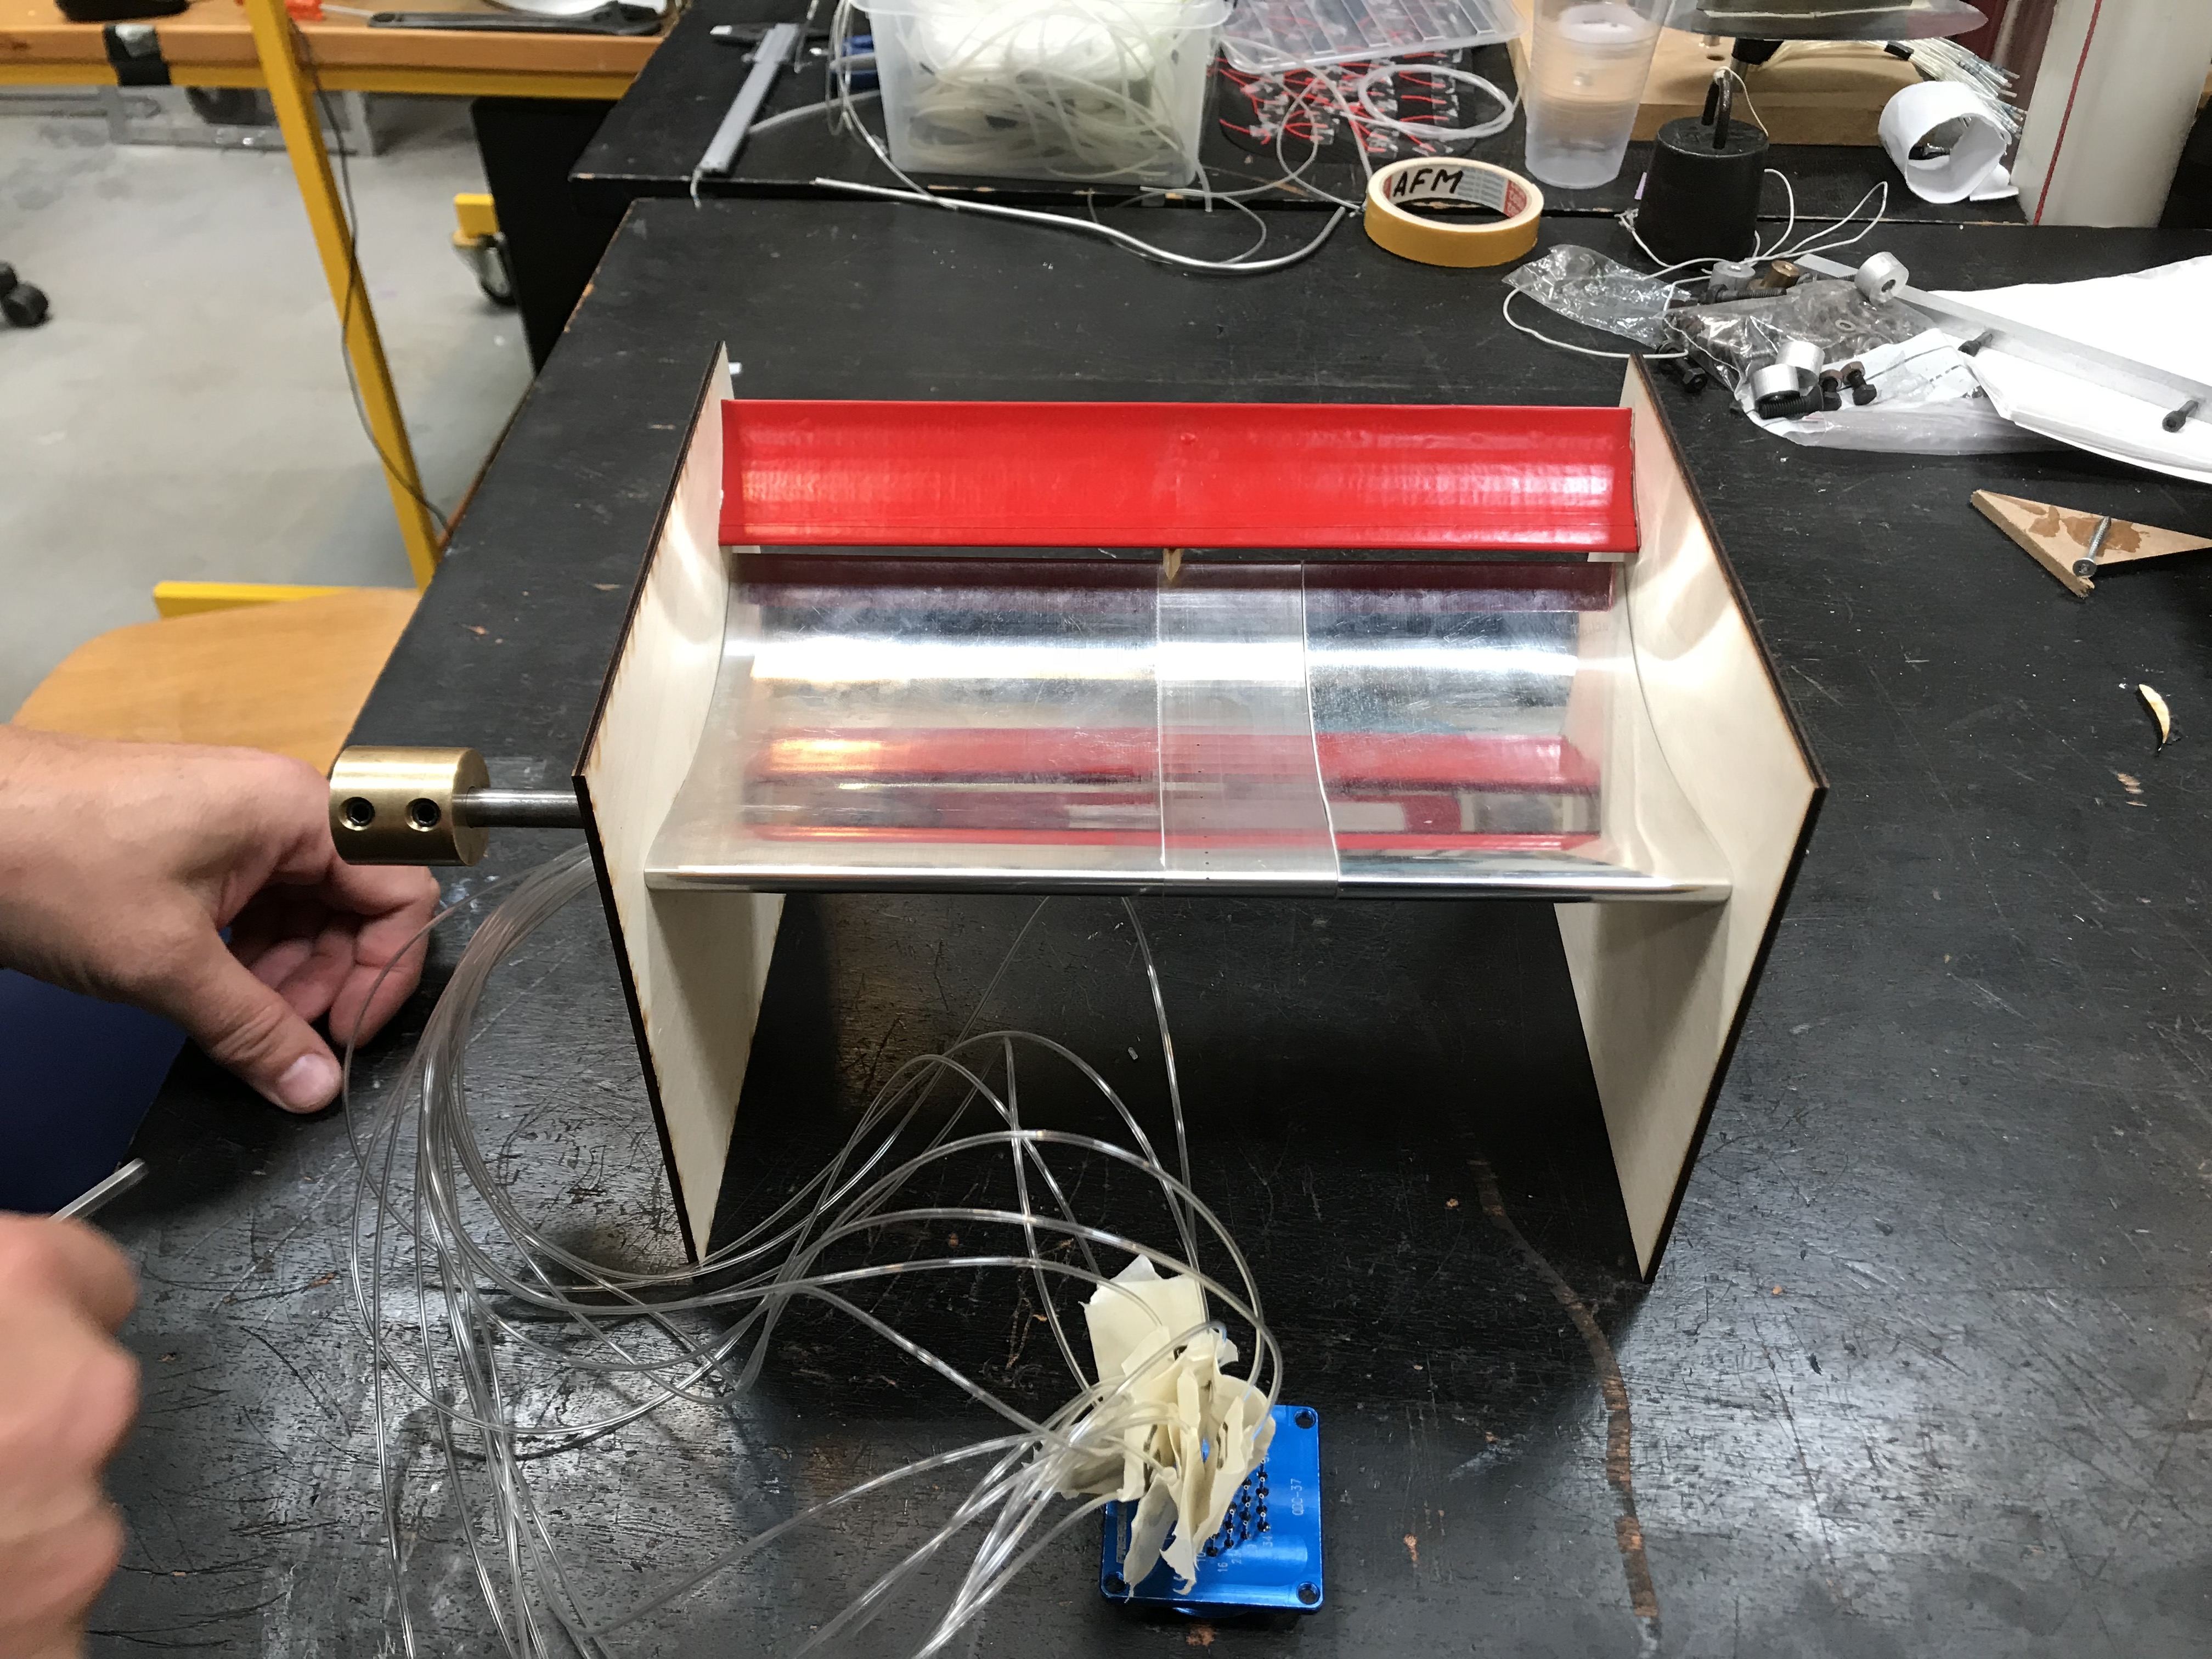
\includegraphics[width=\textwidth]{scalewingAssembled2}
        \caption{Down-scaled wing assmembled with a zoom in on the pressure taps. The length of the entire wing is approximately $\SI{250}{\milli\metre}$ with a total chord length of $\SI{150}{\milli\metre}$.}
        \label{fig:scalewing}
      \end{figure}

      In figure \ref{fig:scalewing} the down-scaled wing post-production with pressure tubes inserted can be seen with pressure-taps along the centerpiece. The wing is assembled by lasercutting the two end plates with holes for mounting, as well as the H7 mounting hole and exits for the pressure tubes.

      In order to strengthen the construction and smoothen the surface, the 3D-printed rearwing was reinforced using tape. The tape is red (as seen in figure \ref{fig:scalewing}), and is additionally supported by a wooden centerpiece holding the two wings together at the right distance. Lastly, the small wing is reinforced further by attaching screws through the end plate, ensuring the wing does not flex.

\section{Experimental Procedure}

  The model wing's $\diameter\SI{8}{\milli\metre}$ hole is fitted with a rod at the end as seen to the left in figure \ref{fig:scalewing}, which is then mounted to the force gauge at he bottom of the wind tunnel. The pressure measurement tubes are passed through a hole in the bottom of the test section, and the pressure rake's height is adjusted to measure the wing's wake. Connection is established to the LabVIEW software running on a nearby computer. A picture of the data collection UI can be found in appendix %\ref{app:labviewview}.

  The wing is positioned with a $0^\circ$ angle of attack. Measurements are taken with $\SI{10}{\metre\per\second}$ increments in the range of $\SIrange{10}{60}{\metre\per\second}$, with an angular sweep at $\SI{20}{\metre\per\second}$ and $\SI{40}{\metre\per\second}$, in order to compare the optimum angle of attack with litterature.

  However, due to the wing covering a relatively large area of the wind tunnel, the final test could only go to $\SI{59.2}{\metre\per\second}$.

  \fxnote{what's the level of obstruction?}

\section{Results}

  The results from the experiment is divided into two parts: A comparison with the theoretical lift values of the downscaled wing, and a comparison with the simulated results. The simulated results will be shown in section \ref{sec:simulationcomparison}, while the comparison to theory can be seen in this section.

  The theoretical lift coefficient at of the scale wing using a total AOA of $\alpha = 35^\circ$, an effective additional AOA from the wing's camber of $\alpha_{L_0} = 0^\circ$ CITE SOMETHING HERE and equation \cite{eq:CL} is found to be:
  \begin{align*}
    C_L &= \left(\frac{2\pi}{1+\frac{2}{\frac{b}{c}\left(1+1.9\frac{h}{b}\right)}}\right)\left(\alpha + \alpha_{L_0}\right)\\
    &\Rightarrow
    \left(\frac{2\pi}{1+\frac{2}{\frac{\SI{250}{\milli\metre}}{\SI{155}{\milli\metre}}\left(1+1.9\frac{\SI{175}{\milli\metre}}{\SI{250}{\milli\metre}}\right)}}\right)\left(\frac{35\pi}{180}\right) = 2.51
  \end{align*}

  Comparing the theoretical lift to the lift coefficients found by the experiments is seen in figure \ref{fig:clperAOAexperiment}. The purple line is the theoretical lift, where the wing's angle is swept between $-10^\circ$ and $10^\circ$. The measured lift is slightly lower than the theoretical, which may be explained by the end plate's effect on aspect ratio. The downscaled wing has a very large $\AR$, where the end plates extend far below the bottom of the wing. While theoretically positive, the effect of the long end plates might not extend all the way up to the wing profile, artificially inflating up the theoretical lift number.

  \begin{figure}
    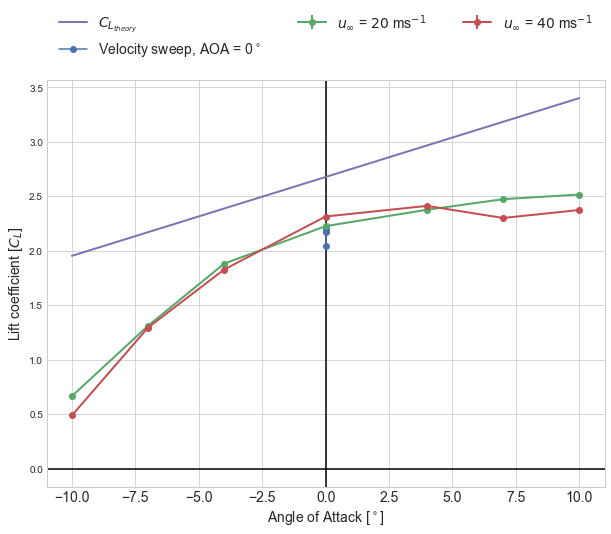
\includegraphics[width=\textwidth]{clperAOAexperiment}
    \caption{The lift coefficient plotted as a function of the wing's overall AOA. The wing's own angle of attack is $35^\circ$, which is beyond the theoretical optimum as seen in figure \ref{fig:AOAofairfoils}.}
    \label{fig:clperAOAexperiment}
  \end{figure}

% !TEX root = main.tex
\chapter{Simulation}
\label{chap:simulations}

  The simulation will run in several parts. First, the wings relative placement between each other will be optimized in a 2-dimensional environment. This involves, $x$- and $y$-distance between the multi-element wings, angle of attack and height relative to the chassis to give a good estimate of the wings placement range. Secondly, a 3-dimensional analysis of the entire wing with endplates will be performed. Endplate dimensions will be optimized, and further optimization of the height relative to the entire chassis to finalize the design and placement.

\section{Star-CCM+}
  Star-CCM+ was used to run the simulations of the wing first in the windtunnel for verification and next on a model of the full size wing to produce an estimate of the performance at full scale. As meshing and running the simulations were heavy computational tasks, the computations were run on the \emph{Niflheim Linux cluster supercomputer}, which is installed at the Department of Physics at DTU.

  The program numerically solves the Navier-Stokes equations, which are derived by the conservation of energy, mass and momentum through a volumetric flow. As Star-CCM+ uses the finite volume method, the equations are discretized to the conservative form: The in- and outgoing flux through a control volume must be conserved. Mathematically, this is expressed as:

  \begin{align}
    \frac{\delta}{\delta t} \iiint Q dV + \iint F dA = 0
  \end{align}
  Where $Q$ is the vector of the conserved variables (eg. $\rho =$ density), $F$ is the vector of fluxes(eg. $\rho u =$ mass flux, $\rho u^2 + p=$ momentum flux + pressure force) and $V$ is the control volume element and $A$is the surface area of the control volume element. The turbulence model Star-CCM+ employs is a K-epsilon turbulence model which is the most commonly used in computational fluid dynamics. %The equations Star-CCM+ solves are the turbulent kinetic energy $k$:
  %\begin{align}
  %  \frac{\delta (\rho k)}{\delta t} + \frac{\delta (\rho k u_i)}{\delta x_i} &= \frac{\delta}{\delta x_j} \left(\frac{\mu_t}{\sigma_k}\frac{\delta k)}{\delta x_j}\right) + 2\mu_t E_{ij}E_{ij}-\rho \epsilon
  %  \intertext{and the dissipation $\epsilon$:}
  %  \frac{\delta (\rho \epsilon)}{\delta t} + \frac{\delta (\rho \epsilon u_i)}{\delta x_i} &= \frac{\delta}{\delta x_j} \left(\frac{\mu_t}{\sigma_\epsilon}\frac{\delta \epsilon)}{\delta x_j}\right) + C_{1\epsilon} \frac{\epsilon}{k} 2\mu_t E_{ij}E_{ij}-C_{2\epsilon}\rho \frac{\epsilon^2}{k}
  %\end{align}

  The interested reader of how Star-CCM+ works is referred to the \emph{User Guide Star-CCM+, version 13.02}.

\section{Mesh Generation}
\label{sec:mesh}
  The mesh has to be structured in accordance to best practice. Areas with high velocity and pressure gradiants have to be dissolved in acceptable resolutions, in order to ensure correct results. Running an initial test on a generic mesh made it clear where the volumemesh requires greater resolution. Gradiants are easily visible around the wing's leading edge, and generally around the solid bodies. Furthermore, aligning the mesh with the flow improves accuracy and rate of convergence. To determine the convergence of simulation results six different mesh resolutions where used to examine the simulations for the windtunnel setup with a wind velocity of $\SI{40}{\metre\per\second}$. Finding the minimum mesh resolution where results have converged with higer resolution results, means a minimum computation time can be achived and thereby allowing for more simulations to be run.

  \begin{figure}
    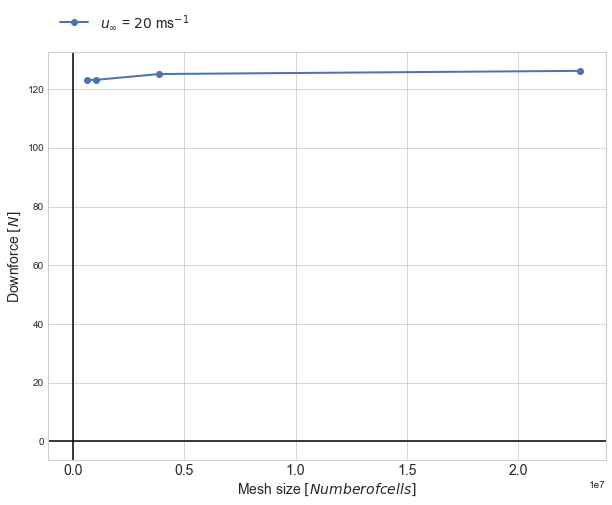
\includegraphics[width=\textwidth]{DFprmeshsize}
    \caption{Normalized downforce as a function of mesh size. Plotted to see the convergence towards the same force.}
    \label{fig:DFprmeshsize}
  \end{figure}

  Generating a mesh of correct size is done by sampling downforce over a range of mesh sizes. In figure \ref{fig:DFprmeshsize}, the normalized downforce is plotted as a function of the mesh size. The mesh independence study shows that the function converges to acceptable levels near the mesh size $\SI{.4E7}{}$, and serves to be a good compromise between results and computing time.

\section{Optimizing the Rear Wing}

  As mentioned in chapter \ref{chap:conceptdesign}, there's a large variation in parameters to optimize for. Numerical optimization has been done on end plates size and relative position of the two wing elements.


  \subsection{Verification of Simulation Results}
  \label{sec:simulationcomparison}

  The data from the experimental test with the $\frac{1}{4}$ scale was first plotted to obtain a picture of the surface pressure on the test wing. An example of a mean over 3000 pressure readouts for a wind speed of $\SI{40}{\metre\per\second}$ is shown in figure \ref{fig:surfacepressureint}, with the standard deviation shown as errorbars. Measurements were run in wind tunnel from $\SI{10}{\metre\per\second}$ to $\SI{60}{\metre\per\second}$ in steps of $\SI{10}{\metre\per\second}$.

  \begin{figure}
    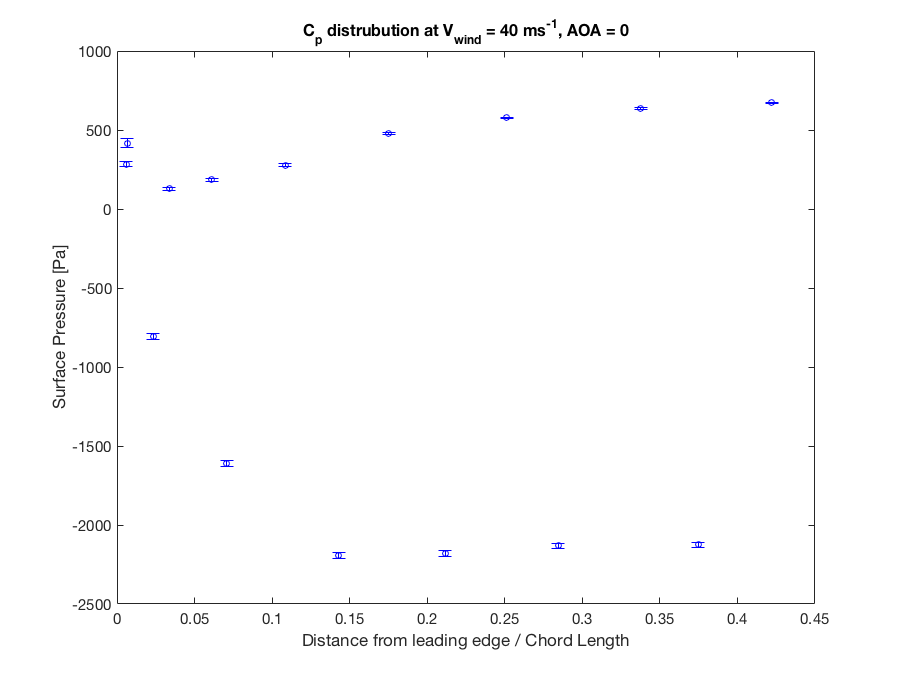
\includegraphics[width=\textwidth]{surfacepressureint}
    \caption{Surface pressure readout from the 15 pressure taps at wind speed $\SI{40}{\metre\per\second}$ in the wind tunnel. Pressure readout is meaned over 3000 measurements and shown with errorbars representing the standard deviation of the measurements.}
    \label{fig:surfacepressureint}
  \end{figure}

  Simulations were then run in \emph{Star-CCM+}. Firstly the CAD model of the $\frac{1}{4}$-scaled wing was imported in the software, then the dimensions of the Red wind tunnel was drawn and the CAD model was placed in the same location as in the real tunnel test. The setup was then volume mesheded with a cell count of around $0.4 \cdot 10^{7}$ million cells as found in section \ref{sec:mesh}. A 2D view of the 3D mesh is shown in figure \ref{fig:mesh3point8mill}. After meshing the physics model for the simulation is set, and simulations are run for the different wind velocities.

  \begin{figure}
    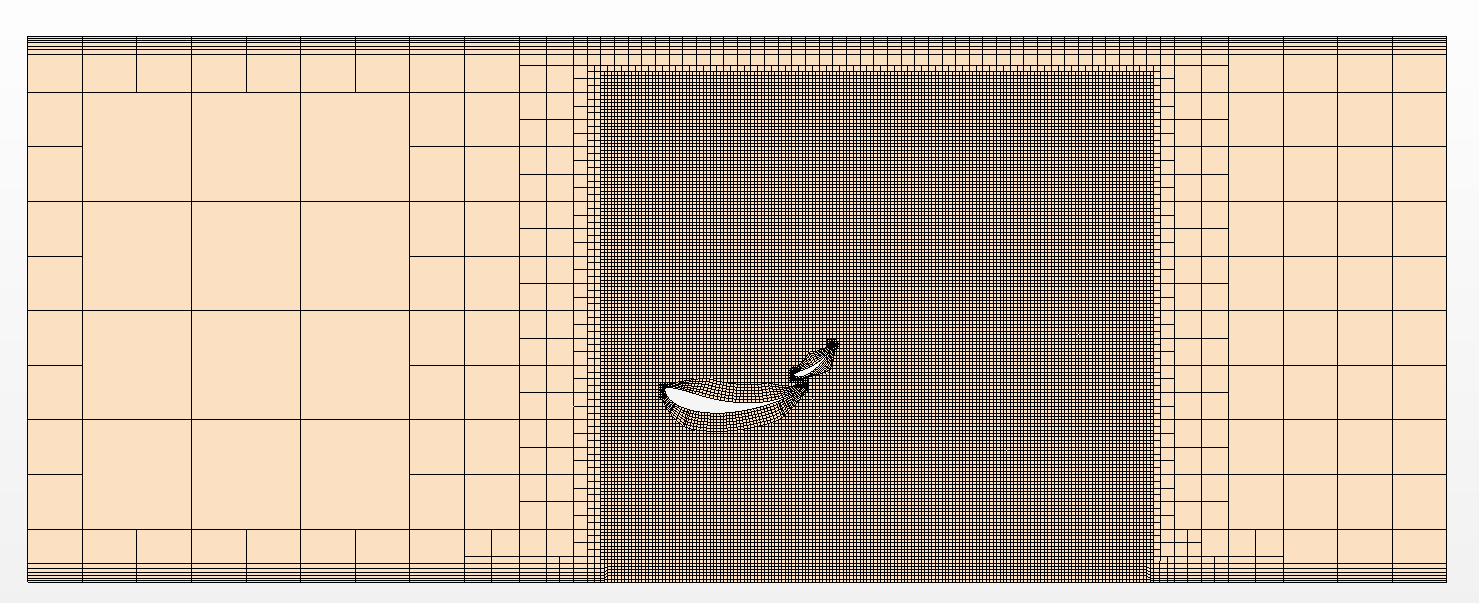
\includegraphics[width=\textwidth]{mesh3point8millcells}
    \caption{2D cut through of the 3D mesh used for simulations of the wind tunnel test.}
    \label{fig:mesh3point8mill}
  \end{figure}

  The simulations are run until the simulation reseults converges to a result. Monitors of the dragforce and downforce for the wing found by the simulation were used to the convergence of the results, an example is shown in figure \ref{fig:downforcemonitor}. Furthermore scalar views and vector views of the pressure distribution and wind velocity around the wing profile can visually help verify that the solutions does not have any obvious faults, such as areas with extremly high velocity og pressure indicating the solutions is not realistic. Examples of a scalar view for the pressure distribution and a vector view of the wind velocity are shown in \ref{fig:pressureScalarV40} and \ref{fig:velocityScalarV40}.

  \begin{figure}
    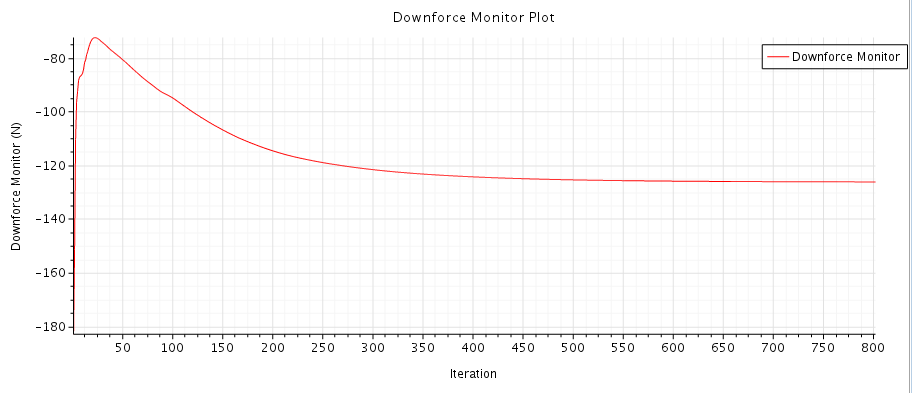
\includegraphics[width=\textwidth]{downforcemonitor}
    \caption{Monitor of the convergence of the downforce over the number of iterations in Star-CCM+, here shown for a wind velocity of $\SI{40}{\metre\per\second}$.}
    \label{fig:downforcemonitor}
  \end{figure}

  \begin{figure}
    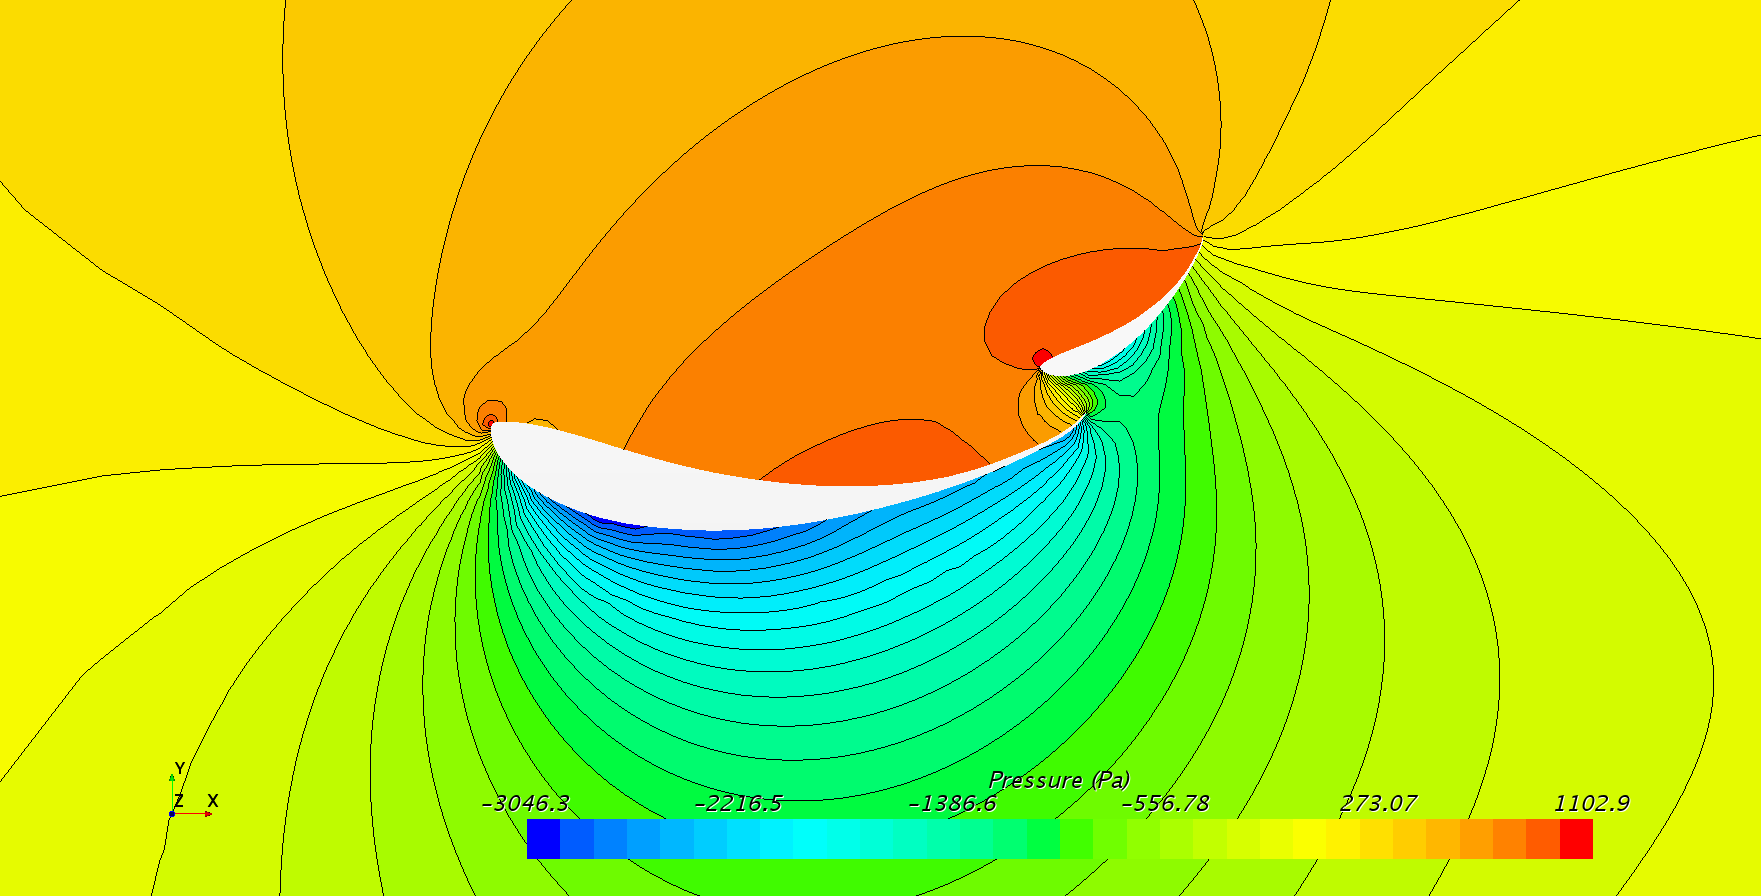
\includegraphics[width=\textwidth]{pressureScalarV40}
    \caption{Scalar view of the pressure distribution surrounding the two elements of the wing, here at a wind velocity of $\SI{40}{\metre\per\second}$.}
    \label{fig:pressureScalarV40}
  \end{figure}

  \begin{figure}
    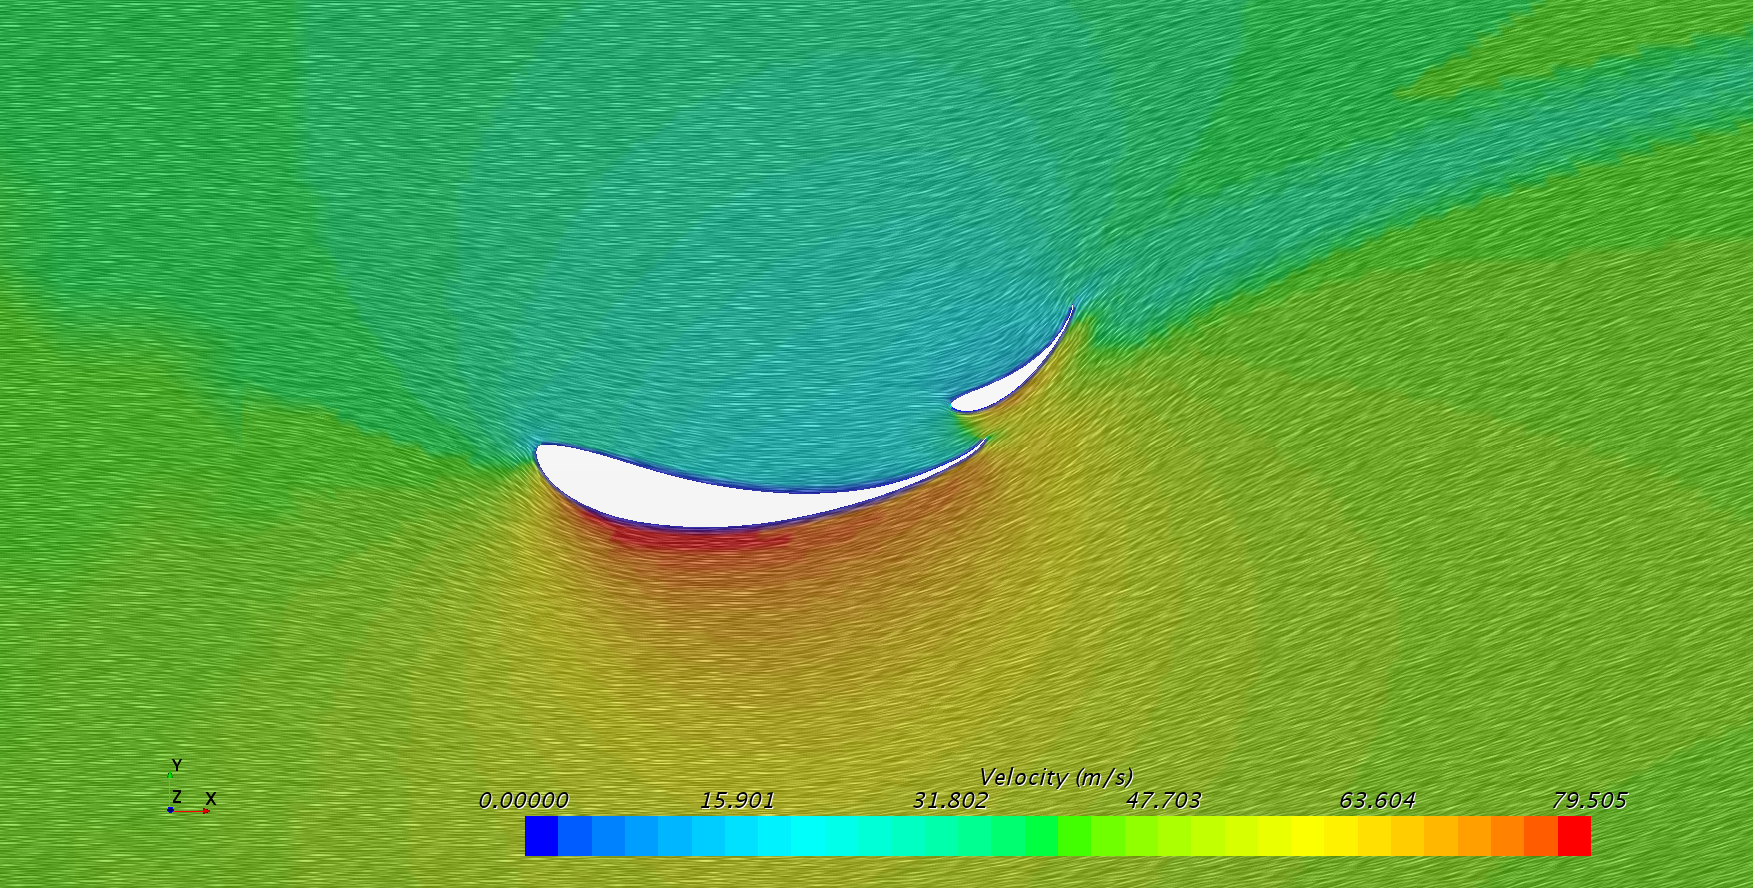
\includegraphics[width=\textwidth]{velocityScalarV40}
    \caption{Vector view of the wind velocity surrounding the wing, here at a wind velocity of $\SI{40}{\metre\per\second}$.}
    \label{fig:velocityScalarV40}
  \end{figure}

  From the simulations the surface pressure of the airfoils was also found, and saved to compare with the measurements of the surface pressure from the real wind tunnel test. The simulated surface pressure is shown in figure \ref{fig:simsurfacepressurev40}.

  \begin{figure}
    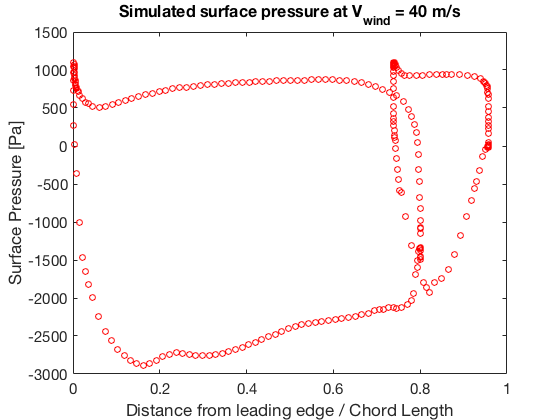
\includegraphics[width=\textwidth]{simsurfacepressurev40}
    \caption{Simulated surface pressure on both elements of the wing. To the left the larger element surface pressure and the smaller elements surface pressure is shown right. Simulated at wind velocity of $\SI{40}{\metre\per\second}$.}
    \label{fig:simsurfacepressurev40}
  \end{figure}

  Comparing the surface pressure predicted by the simulation,\ref{fig:simsurfacepressurev40}, and measured in the test, \ref{fig:surfacepressureint}, show that two are not i sync. Comparing the predicted downforce and measured downforce, shows that the simulated results predict a $\SI{40}{\%}$ downforce than measured. This could be caused by several factors. One factor could be the assembly of the test wing is not a perfect replica of the full scale wing, an improement to help this would be by producing the scaled model completely by machining with small tolerances, compared to the half machined and half handbuild model used in these test. This could cause the relative position of the 2 wing elements to be diffrent from the CAD model used in simulations.

  Finding the correct correlation between the estimated downforce and extact surface pressure will not be possible in this report. The simualtions and measurements can however be compared by using the dimensionless number, the pressure coefficient,

  \begin{align}
    C_p \equiv \frac{p-p_{\infty}}{\frac{1}{2}\rho_{\infty}V_{infty}^2},
  \end{align}

  where $p$ is the static pressure at the point being evaluated, $p_{\infty}$ is the static pressure in the freestream, $\rho_{\infty}$ is the freestream fluid density and $V_{\infty}$ is the freestream velocity of the fluid. The pressure coefficient describes the relative pressure throughout a fluid in movement. In many situations the pressure coefficient near a body is independt of the size of the body. \fixme{Consider moving to theory}

  The pressure coefficient allows us to compared the form of the relative pressure between the simulations and the experimental test. This comparison is shown in figure \ref{fig:CpV40}. When comparing the two, a difference in value is still visible due to the difference in absolute pressure, but the form of the two $C_p$ distributions, confirm the characteristics of the flow around the wing is uptain through the simulation. A higher resolution of measuring taps would help further testing, but for the smaller model is very difficult to achieve due to lack of space. \fixme{fix labels. fixed}

  \begin{figure}
    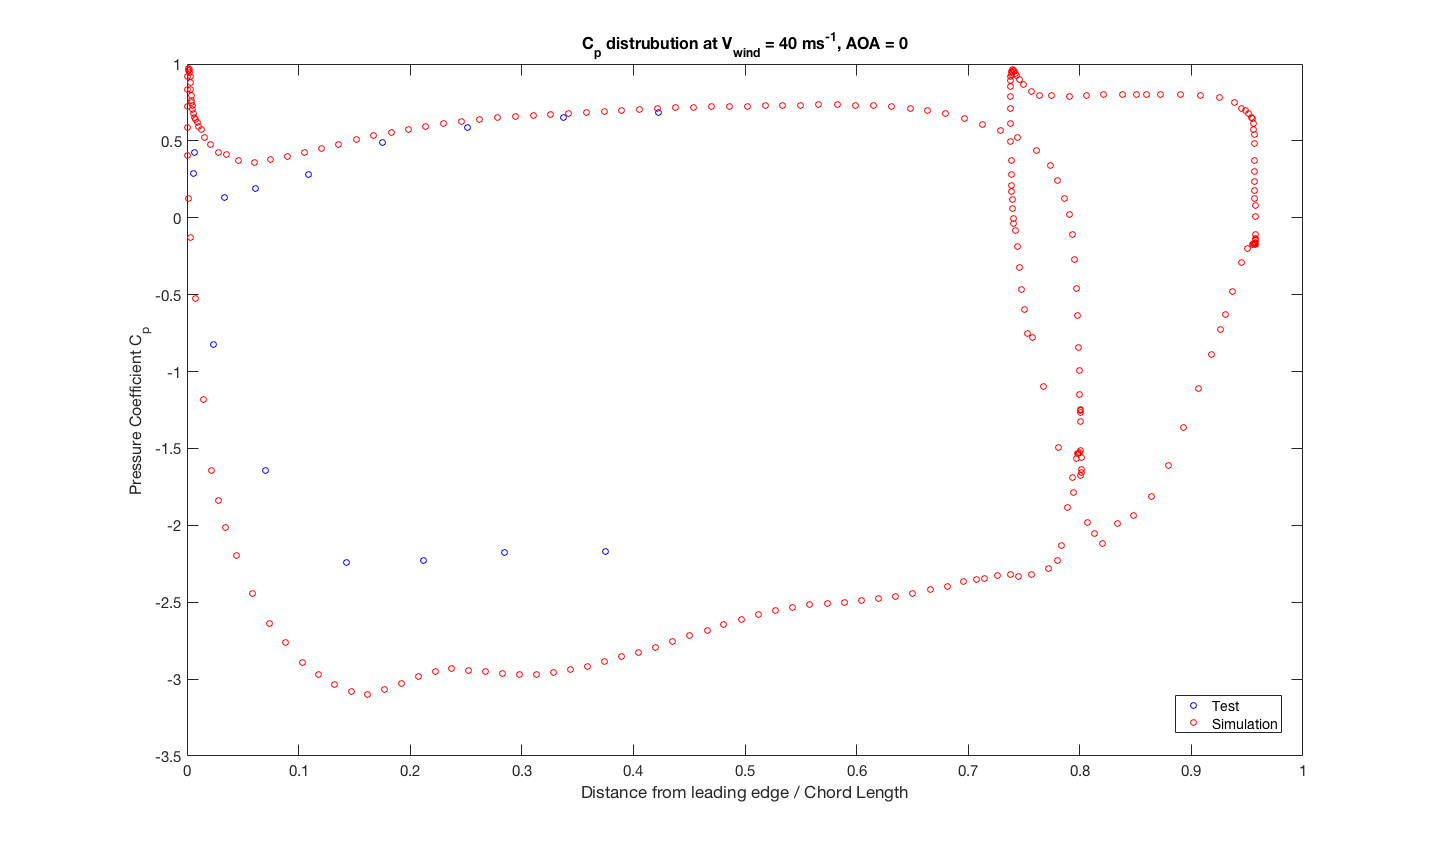
\includegraphics[width=\textwidth]{CpV40}
    \caption{Comparison of simulated and test found $C_p$ values at a wind velocity of $\SI{40}{\metre\per\second}$.}
    \label{fig:CpV40}
  \end{figure}

  The use of simulations for designing an aerodynamic package for the race car for the moment is usefull as a way to insure the realtive pressure distrubtion aorund the wing is as wanted, and ensuring that the flow does not seperate at unwanted locations. However further work on the correlation between simulated downforce and measured downforce is still needed and the work will continue with the Vermilion Racing team, in order to have the best possibilities to design a good aero-package before having to build it.

  Lastly worth noting is when the simulated flow is visualized by streamlines, the vortex generation at the rear of the wing, as mentioned in section \ref{subsec:endplates}, is shown clearly in figure \ref{fig:simvortex}. It is clear that the size of the produced vortices are interacting with the side walls of the wind tunnel. A sugestion for further testing of an wing with such large vortex generation would be to use a wind tunnel with a larger cross-secton to avoid interactions with the side walls.

  \begin{figure}
    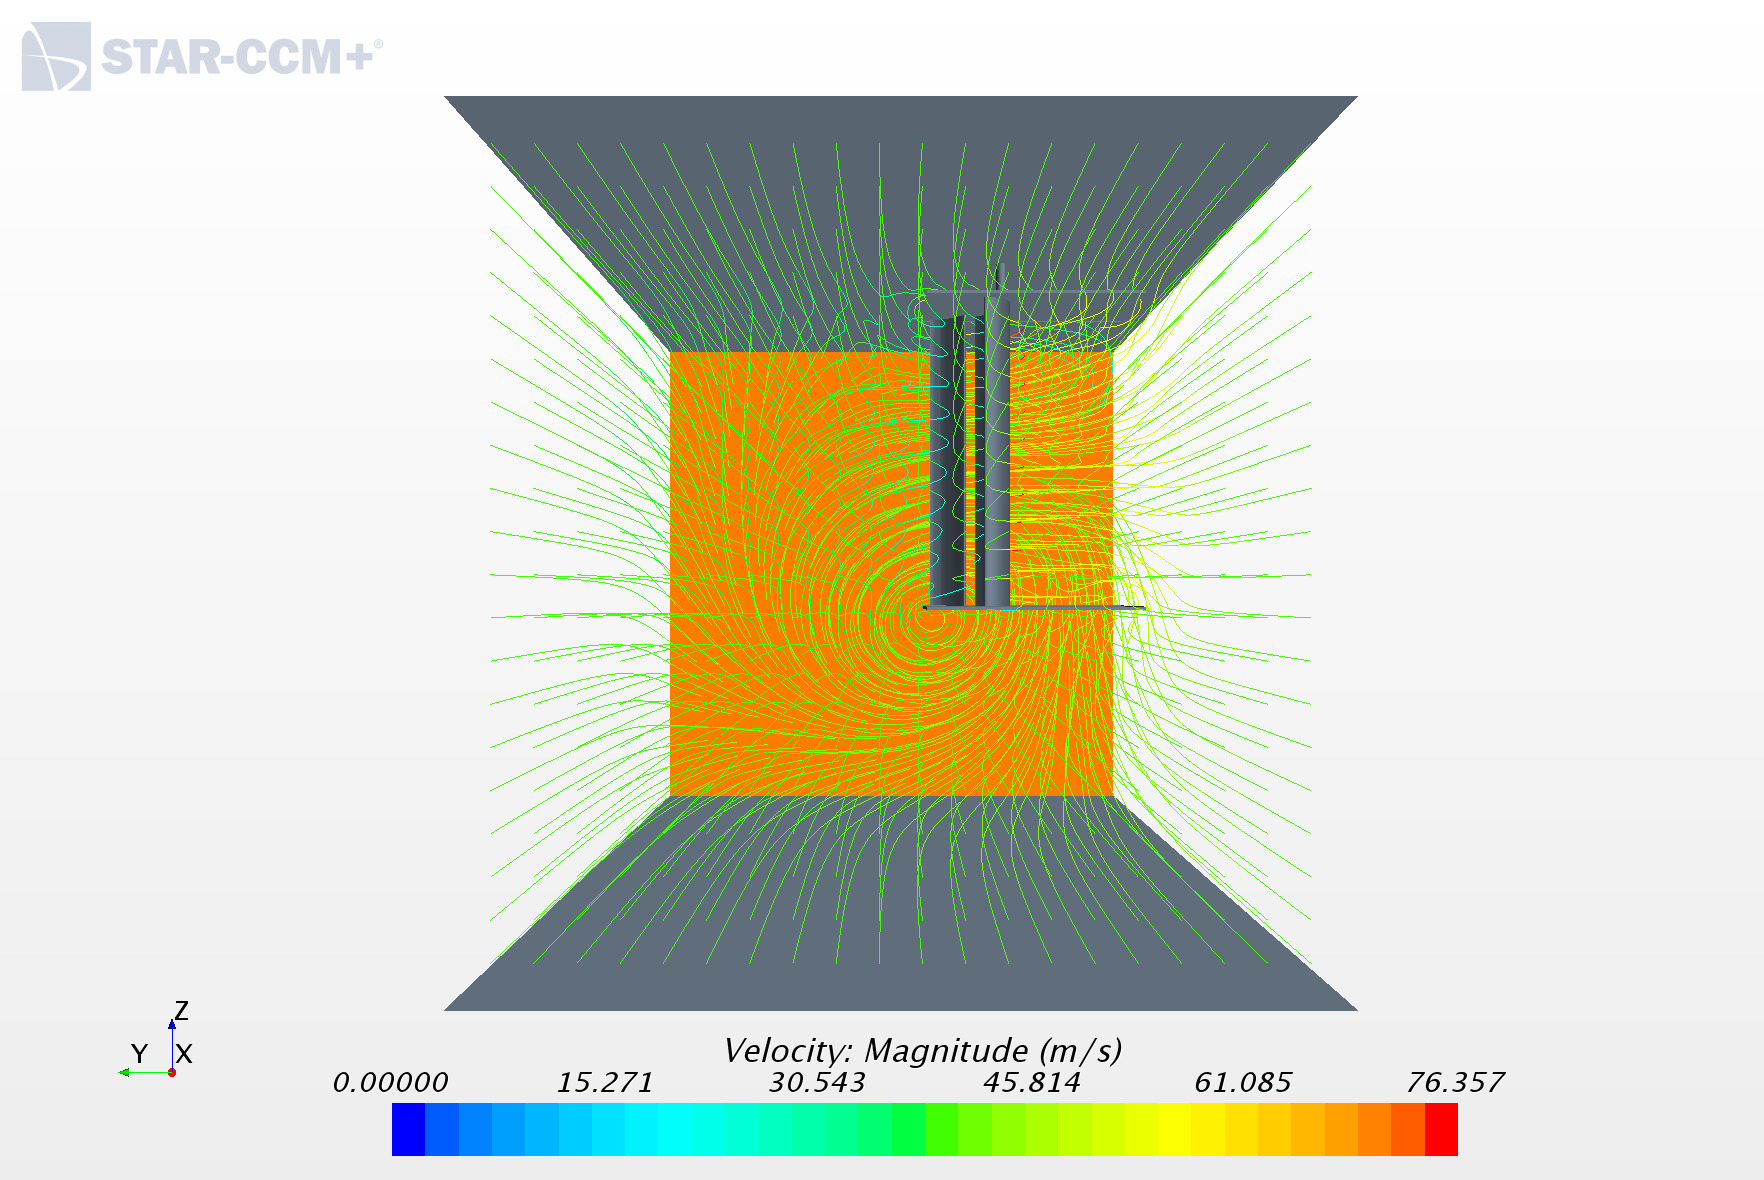
\includegraphics[width=\textwidth]{simulatedvortex}
    \caption{Visualization by streamlines of the simulated airflow around the wing. Vortex generation at the rear of the wing is visiable.}
    \label{fig:simvortex}
  \end{figure}

  \subsection{Multi-Element Wing Optimization}
  The influence of the two wing elements relative position on lift was examined to optimize the downforce the rear wing provides to the car at a given velocity. This relative position optimization was performed in the software package \emph{MultiElements Airfoils} provided from \emph{Hanley Innovations}. A scatterplot of the relative position is seen in figure \ref{fig:multieleoptimization}. The trailing edge of the first element is seem as the dark lines, and the position of the second elements leading edge is plotted, where the resulting lift coefficient is embedded as color. The redder the better lift coefficient. After sweeping, a maximum lift of $C_L = 2.60$  at $u = \SI{15}{\metre\per\second}$. is found with the leading edge of the secondary element placed at $x=\SI{0.5}{\metre},y=\SI{-0.01}{\metre}$ relative to the leading edge of the main element.

  \begin{figure}
    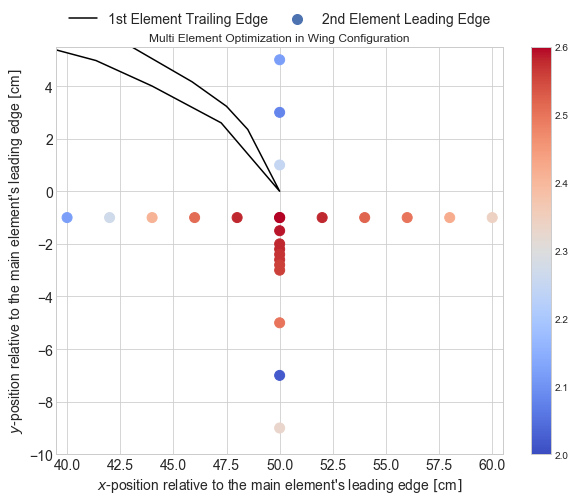
\includegraphics[width=\textwidth]{multieleoptimization2}
    \caption{Optimization of the two element wing. The redder the dots, the higher the lift coefficient.}
    \label{fig:multieleoptimization}
  \end{figure}

\section{Downforce Estimate of Full Scale Wing}
\fixme{Maybe save for defense}

\include{construction}
% !TEX root = main.tex
\chapter{Discussion}
  The following section will discuss the results in chapter \ref{chap:experiments} and the simulations made in chapter \ref{chap:simulations}. The purpose of this paper was to investigate the effects or aerodynamics on race cars, design a solution that would improve the car's lap time and finally produce the hypothesized aerodynamic device.

  \section{Theory, Experiments and Simulations}

  The wind tunnel results plotted in figure \ref{fig:clperAOAexperiment} shows a correlation between the wing's lift and theoretical lift, assuming a constant $C_L$ for the theoretical wing. The experimental results are all lower than the theoretical, which may be due to several facts: First, the wing section's alignment at higher speeds was interrupted, as one section was skewed $\SIrange{2}{3}{\milli\metre}$, creating a small gap between the wing sections. Secondly, the wing's extremely high lift interferes with the flow behaviour, as the wing's wake is most likely pushing air against the walls. This theory is corroborated by the simulations as seen in figure \ref{fig:scalewingwindtunnelsim}, where it is clearly seen that the wake interferes with the wall's boundary layer. Third, and most likely the most important, the placement relative to each other may be slightly off. Creating a small multi element airfoil is very difficult, as placement is everything to the lift of the wing. According to the wing optimization process seen in figure \ref{fig:multieleoptimization}, very small changes can rapidly change the  lifting characteristics of the wing. This could explain why the lift of the airfoil model is much lower than the theoretical, and the fact that the simulations coincide very well with theory.

  After evaluating the experimental results and the simulations, it was clear that theory sided with the simulations. This evoked an investigation of the down scaled wing model, revealing a relative position of the trailing-edge-to-tip position of $(x,y) = (\SI{-11.5}{\milli\metre},\SI{-8}{\milli\metre})$, instead of the planned $(\SI{-6.9}{\milli\metre},\SI{-12.5}{\milli\metre})$. The variation comes from placing the wing initially. The importance of the position was not uncovered until simulations optimizing their relative position, and due to time the experiment was not redone. However, a simulation using the new relative position of the wing was performed, showing a change in lift from $ C_L = 2.50 \rightarrow 2.43$ due to misplacing the second element. Additionally, the angle of the second element is of great importance to the lift, removing in the excess of $20\%$ of the lift coefficient if wrongly placed. The lesson learned is that the second element must be very carefully placed relative to the first element, in order to not alter the flow substantially.

\section{Product Design Specification Review}

  The finished product have to live up to the design specification, in order to be a useful solution. In table \ref{tab:designreview}, it can be seen that all reqirements are fulfilled, and all criteria except one. During the design process of the car, the removal of the engine became negligible as the battery pack is going to be removed in another way. This voids the criteria, and thus makes the solution an optimal one.

  \begin{table}
    \begin{tabularx}{\textwidth}[t]{>{\columncolor{seapurple!40}}l XX}
      \arrayrulecolor{seapurple}\hline
      \rowcolor{white}
      \textbf{\textcolor{seapurple}{Issue}} & \textbf{\textcolor{seapurple}{Requirement}} & \textbf{\textcolor{seapurple}{Criteria}}\\
      \hline
      Weight & \cellcolor{seagreen!40}Must not move CM above halfway point & \cellcolor{seagreen!40}Should be as low as possible \\
      Safety & \cellcolor{seagreen!40}Must be in compliance with FSAE rules & \cellcolor{seagreen!40}Should not make handling difficult for driver\\
      Durability & \cellcolor{seagreen!40} Must have no fatigue limit. Must to be waterproof \\
      Performance & \cellcolor{seagreen!40} High downforce \& soft stall characteristic at all speeds &\cellcolor{seagreen!40} Should retain perfomance despite tripping. Should have end plates.\\
      Dimensioning & \cellcolor{seagreen!40} Must be within area defined by FSAE rules & \cellcolor{seayellow!40} Should allow space for motor removal. \\
      Production & \cellcolor{seagreen!40} Low time- and monetary cost
      \label{tab:designreview}
    \end{tabularx}
    \caption{The PDS table shows how the final design lives up to the proposed specifications.}
  \end{table}

  \section{Factual Improvements}

  The theoretical lift coefficient found from simulations is shown to be $C_L = -2.8$. For a complete lap time simulation the entire aerodynamics package has to be finished. Numbers from the initial calculations of the front wing and undertray provide an estimated total lift coefficient of the car to be around $C_L = -2.4$ \cite{lcdesign}. As seen in figure \ref{fig:cornerspeedvsliftrelative}, this should increase the tight cornering speed from with $4-5\%$, while for larger radius corners upwards $20-45\%$!

  \begin{figure}
    \makebox[\textwidth][c]{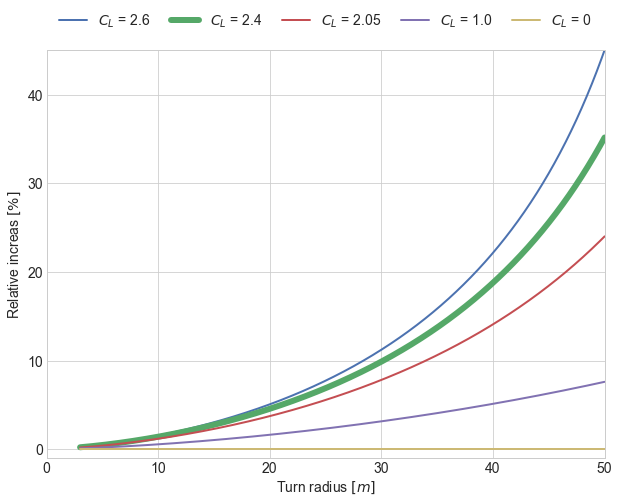
\includegraphics[width=1.2\textwidth]{turnspeedperCLrelative}}%
    \caption{Cornering speed as a function of turn radius for various lift coefficients, relative to a $C_L = 0$.}
    \label{fig:cornerspeedvsliftrelative}
  \end{figure}


  %Based on equation \ref{eq:downforcetocorneringspeed}, the cornering speed due to the added downforce of the wing can be found to give
  %\begin{align}
%    \dot{x} &< \left(\frac{r}{m} \mu (mg + F_L)\right)^{\frac{1}{2}}
%    \intertext{which for a  turn }
%  \end{align}

  While fulfilling the PDS, the ease of prodution and being a first design ever restricted the scope of the project. Great improvements can be expected in the coming years. The extend of the theory required in order to produce a rear wing has been uncovered, and this project serves as a guide line for future iterations of the rear wing.  In chapter \ref{chap:perspective}, a series of possible improvements are evaluated and proposed for increasing the aerodynamic contribution to increasing lap times.

% !TEX root = main.tex
\chapter{Conclusion}

% !TEX root = main.tex
\chapter*{Perspective}
\label{chap:perspective}

The Eevee has to be rebuilt next year, and in order to help the effort along for future students, a list of potential upgrades are listed below, with estimates of how valuable each change is in regards to downforce/drag reduction gain.

\section{Drag Reductive System}

A drag reductive system (DRS) is well-known from Formula 1, and has in the recent years been gaining traction (or lack therof :))) ) in the Formula Student. It is a natural extension to the aerodynamics of the car, as Formula Student has much less restrictions on aerodynamics than Formula 1. Automatically adaptive DRS, that measures the car's relative downforce and the angle of the steering column could give a big edge on straights, as flipping the wing up to reduce drag increases the top speed.

\section{Slats, Flaps, Gills and Cutaway}

https://www.jmranalytical.com/single-post/2017/04/06/Rear-Wing-Investigation

We already have a multi element wing, but increasing the amount of elements increases the amount of downforce we can pull out of the same design.

\section{Suspension Integration}

- Nice to have downforce directly on the wheels
- Gives more unsprung mass though. That might be an issue.

% !TEX root = main.tex
\chapter*{Media}

The project gained a lot of media attraction. For the interested reader, more can be found below.

% !TEX root = main.tex
\begin{appendices}
\chapter{Appendix}
\newpage
\section{Appendix A:LabVIEW program}
\begin{figure}
  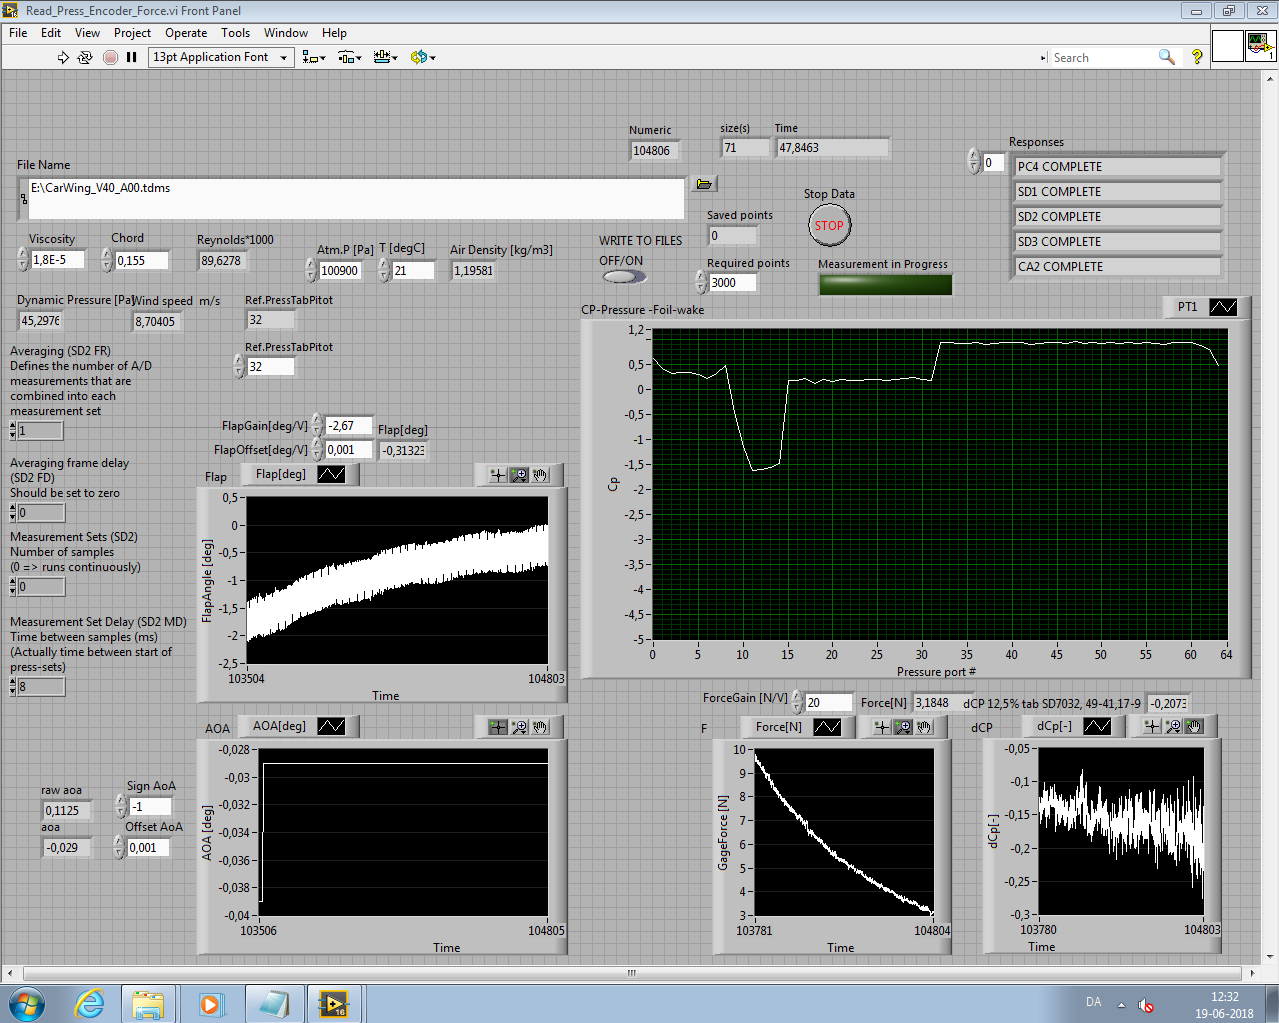
\includegraphics[height = 0.75 \textheight]{labviewview}
  \caption{Picture of the LabVIEW program used to receive data}
  \label{app:labviewview}
\end{figure}

\chapter{Carbon Fiber Data Sheet}
\label{app:carbonfiberdatasheet}
\chapter{Hardener Data Sheet}
\label{app:hardener}
\chapter{Resin Data Sheet}
\label{app:resin}
\end{appendices}


%%%%% BIBLIOGRAPHY %%%%%
\nocite{*}
\bibliographystyle{unsrt}
\bibliography{references}
\end{document}
